%%%%%%%%%%%%%%%%%%%%%%%%%%%%%%%%%%%%%%%%%%%%%%%%%%%%%%%%%%%%%%%%%%%%
%% I, the copyright holder of this work, release this work into the
%% public domain. This applies worldwide. In some countries this may
%% not be legally possible; if so: I grant anyone the right to use
%% this work for any purpose, without any conditions, unless such
%% conditions are required by law.
%%%%%%%%%%%%%%%%%%%%%%%%%%%%%%%%%%%%%%%%%%%%%%%%%%%%%%%%%%%%%%%%%%%%

\documentclass[
  digital, %% The `digital` option enables the default options for the
           %% digital version of a document. Replace with `printed`
           %% to enable the default options for the printed version
           %% of a document.
%%  color,   %% Uncomment these lines (by removing the %% at the
%%           %% beginning) to use color in the printed version of your
%%           %% document
  oneside, %% The `oneside` option enables one-sided typesetting,
           %% which is preferred if you are only going to submit a
           %% digital version of your thesis. Replace with `twoside`
           %% for double-sided typesetting if you are planning to
           %% also print your thesis. For double-sided typesetting,
           %% use at least 120 g/m² paper to prevent show-through.
  lof,     %% The `lof` option prints the List of Figures. Replace
           %% with `nolof` to hide the List of Figures.
  lot,     %% The `lot` option prints the List of Tables. Replace
           %% with `nolot` to hide the List of Tables.
]{fithesis4}
%% The following section sets up the locales used in the thesis.
\usepackage[resetfonts]{cmap} %% We need to load the T2A font encoding
\usepackage{latex-javaScript/jslistings}
\usepackage[T1,T2A]{fontenc}  %% to use the Cyrillic fonts with Russian texts.
\usepackage[
  main=english, %% By using `czech` or `slovak` as the main locale
                %% instead of `english`, you can typeset the thesis
                %% in either Czech or Slovak, respectively.
  english, german, russian, czech, slovak %% The additional keys allow
]{babel}        %% foreign texts to be typeset as follows:
%%
%%   \begin{otherlanguage}{german}  ... \end{otherlanguage}
%%   \begin{otherlanguage}{russian} ... \end{otherlanguage}
%%   \begin{otherlanguage}{czech}   ... \end{otherlanguage}
%%   \begin{otherlanguage}{slovak}  ... \end{otherlanguage}
%%
%% For non-Latin scripts, it may be necessary to load additional
%% fonts:
\usepackage{paratype}
\usepackage{my-alias}
\def\textrussian#1{{\usefont{T2A}{PTSerif-TLF}{m}{rm}#1}}
%%
%% The following section sets up the metadata of the thesis.
\thesissetup{
    date        = \the\year/\the\month/\the\day,
    university  = mu,
    faculty     = fi,
    type        = bc,
    department  = Department of Machine Learning and Data Processing,
    author      = Adam Hlaváček,
    gender      = m,
    advisor     = {RNDr. Vladimír Štill, Ph.D.},
    title       = {Revitalization and Modernization of Web Application of the Epistolary Seminar of Informatics},
    TeXtitle    = {Revitalization and Modernization of Web Application of the Online Seminar of Informatics},
    keywords    = {keyword1, keyword2, ...},
    TeXkeywords = {keyword1, keyword2, \ldots},
    abstract    = {%
      This is the abstract of my thesis, which can

      span multiple paragraphs.
    },
    thanks      = {%
      These are the acknowledgements for my thesis, which can

      span multiple paragraphs.
    },
    bib         = thesis.bib,
    %% Remove the following line to use the JVS 2018 faculty logo.
    facultyLogo = fithesis-fi,
}
\usepackage{makeidx}      %% The `makeidx` package contains
\makeindex                %% helper commands for index typesetting.
\usepackage[acronym]{glossaries}          %% The `glossaries` package
\renewcommand*\glspostdescription{\hfill} %% contains helper commands
\loadglsentries{abbreviations.tex}  %% for typesetting glossaries
\makenoidxglossaries                      %% and lists of abbreviations.
%% These additional packages are used within the document:
\usepackage{paralist} %% Compact list environments
\usepackage{amsmath}  %% Mathematics
\usepackage{amsthm}
\usepackage{amsfonts}
\usepackage{url}      %% Hyperlinks
\usepackage{markdown} %% Lightweight markup
\usepackage{listings} %% Source code highlighting
\lstset{
  basicstyle      = \ttfamily,
  identifierstyle = \color{black},
  keywordstyle    = \color{blue},
  keywordstyle    = {[2]\color{cyan}},
  keywordstyle    = {[3]\color{olive}},
  stringstyle     = \color{teal},
  commentstyle    = \itshape\color{magenta},
  breaklines      = true,
}
\usepackage{floatrow} %% Putting captions above tables
\floatsetup[table]{capposition=top}
\usepackage[babel]{csquotes} %% Context-sensitive quotation marks
\begin{document}
%% Uncomment the following lines (by removing the %% at the beginning)
%% and to print out List of Abbreviations and/or Glossary in your
%% document. Titles for these tables can be changed by replacing the
%% titles `Abbreviations` and `Glossary`, respectively.
\clearpage
\printnoidxglossary[title={Abbreviations}, type=\acronymtype]
\printnoidxglossary[title={Glossary}]

%% The \chapter* command can be used to produce unnumbered chapters:
\chapter*{Introduction}
%% Unlike \chapter, \chapter* does not update the headings and does not
%% enter the chapter to the table of contents. I we want correct
%% headings and a table of contents entry, we must add them manually:

\mdstart

The Online Seminar of Informatics (ESI for short) is an annual online competition and also one of the activities of the Faculty of Informatics targeted at high school students. The central part of ESI takes place from September to April in four thematic waves. Each wave consists of at least a dozen tasks in which the participants can learn and then apply various informatics principles. Participants who earn a minimum of 60\% points for completing given tasks awarded throughout all four waves are suitable to be accepted to the Faculty of Informatics without taking entrance exams. Every year ESI has more than five hundred participants that come to solve the tasks on its current website located at https://ksi.fi.muni.cz/.

The current website is created with an outdated framework, and only a fraction of the current organizers have a needed understanding of possible issues. Because of this, the main goal of this thesis is to create a new web application for ESI, while the main focuses of the new application are on easy and effective moderation in terms of long term support.

Secondary goals of this thesis are for the new web application to make the website usable on mobile devices, present older tasks incompatible with the current website and to improve the overall user experience of the web page.

As a part of this thesis, some related modifications are also made to the server part of the ESI infrastructure.

The first two chapters are dedicated to researching other competitions similar to the ESI and their approach to their websites. The third chapter describes the ESI's server-side infrastructure. Chapter 4–6 illustrates the new implementation. Chapter 7 describes the completed application infrastructure. The resulting web application, which is a primary goal of this thesis, can be seen in use at https://ksi.fi.muni.cz/novy-web/.

\end{markdown*}

\markright{\textsc{Introduction}}
\addcontentsline{toc}{chapter}{Introduction}

\mdchap{Current state of the web frontend of Online Seminar of Informatics}

The current web frontend of the Online Seminar of Informatics (ESI for short) was written using the first version of the Ember.js framework. The last minor version of the first version of the Ember.js framework was released on the 12th of June 2015~[@ember-1]. The frontend stayed principally the same throughout the years because the first Ember.js version cannot be upgraded to a more recent and supported version with ease. Following the fact that Ember v1 was released in 2015, present seminar organizers face a few severe issues -- the foremost being security implications of using old and deprecated software and the secondary being the lack of volunteers with enough knowledge of this technology. In its current state, the frontend is singlehandedly managed by Ondřej Borýsek~[@ksi-web-frontend].

Since the support of the utilized framework ended, the organizers have been aware of these issues. They have tried to migrate the used version to a current stable version of Ember, most notably inside a private project called web-frontend-ember3~[@ksi-web-frontend-ember3], but these attempts were not successful. The leading explanation for the prevalence of the current frontend is that all organizers are volunteers. With only a limited time available, the organizers decided to work on more imminent duties. However, this task has gained a significant priority as Ondřej Borýsek will finish his studies shortly, and, consequently, none of the team members will be capable of resolving issues or implementing new features.

When deciding how to approach the development of the new version of the ESI frontend, I was faced with three viable alternatives. The first option was to adapt the web of any similarly focused seminar, which was deemed inappropriate because the ESI frontend has grown its backend with unique features not easily adaptable from other projects. The second possibility was to continue with a previous attempt to upgrade the frontend to the newer version of the Ember framework. This option was also discarded as there is a risk that the project would be eventually hard to manage, similarly to the current state. As per the Stack Overflow 2020 developer survey~[@stackoverflow-survey], the Ember framework is no longer used regularly and thus unsuitable for a long-lasting project.

The last option was to develop a new project from scratch using one of the most used web frameworks. Besides jQuery, which is not a full-featured web framework, the most used ones are React.js and Angular~[@stackoverflow-survey].

React~[@react-github], developed by Meta, is the most popular~[@stackoverflow-survey] full-featured web framework. It is focused on the fast development of responsive web applications while heavily depending on modularity and supporting it via external libraries. This modularity allows the developer to tailor the project's library set precisely for the project's needs. Since component logic in React.js is written in JavaScript instead of templates, it is easy to pass rich data through the applications and keep state out of the DOM~[@reactjs]. An added benefit of React.js is that it is taught on the Faculty of Informatics Masaryk University in a course Modern Markup Languages and Their Applications, which is compulsory for both
Programming and Development~[@fi-pva] program and some specializations of Informatics~[@fi-inf]. Nevertheless, most of the current members of the organizer teams have no experience with web development whatsoever.

Angular~[@angular], developed by Google, on the other hand, includes most of the frequently used features~[@angular-features] like routing, HTTP client, forms manipulation, and internalization. Therefore Angular allows the developers to get familiar with a new project more rapidly without needing to learn about new libraries used within a given project first.

Because the team of seminar organizers changes quite frequently, it is crucial to minimize the entrance barrier for new developers to be capable of modifying the frontend. A lower entrance barrier can be achieved by using a well-established technology with minimal supplementary knowledge required. Concerning precisely that argumentation, Angular was chosen as more fitting and is utilized throughout this thesis.

\end{markdown*}

\mdchap{ESI Infrastrucute}

ESI's organizers manage two virtual servers hosted on faculty's Open Nebula platform, both running Debian OS. One of these servers is for production, the second is for testing. Both share the same format - an Apache web server, which server the frontend and reverse proxies the backend.
The production server is called `kleobis` and the development `kyzikos` and I will refer to them troughout this thesis as such.

Kleobis has assigned two domains -- [ksi.fi.muni.cz](https://ksi.fi.muni.cz) for access to the frontend and [rest.ksi.fi.muni.cz](https://rest.ksi.fi.muni.cz) for calling backend endpoints.

Kyzikos has no public access, because it is meant as a development server on which the organizers can test their possibly breaking modification without interfering with the production instance.

The frontend~[@ksi-web-frontend] can be automatically deployed from its repository by building it using GitHub Actions and then copying the built web application on the desired server by calling an automated script on one of the organizers faculty accounts.

The backend~[@ksi-web-backend] has no means for automatic deployment and updating. The process has to be performed manualy, by logging into target server, pulling from the source code repository and performing a manual restart. This is a desired workflow, because updates to the backend server are infrequent and a manual check of functionality after an update increases certanity that the server will work as desired even after the update.

## Backend

The backend server~[@ksi-web-backend] is written as a Python 3 project and acts mainly as a middle-ware between the user and the database. A heavily utilized part of the backend is its capability to execute untrusted code sandboxed, which is a crucial part of the ESI. The backend is also capable of manipulating with a git repository containing data of solvable tasks.

### Code sandboxing

To sandbox untrusted code, mainly originating from participants task evaluations, ESI uses `isolate`~[@isolate] project. This project was developed for the needs of programming contests, so it perfectly fits ESI's needs. It uses so-called boxes, in which an executed command has only a limited, but fully defined, set of capabilies. This can mitigate the risk of overloading the host's system by a program stuck in nevereding loop, using the hosts network as a point of entry for an attacker, or even gaining direct access to the hosts system.

### Python web framework

The ESI backend utilizes the Falcon~[@falcon] framework for handling all HTTP API calls, which is used by companies like PayPal and LinkedIn~[@falcon-usage]. This framework is optimized for creating RESTful~[@rest] API and as such is better suitable for larger volume of incoming requests. Every endpoint is defined as a class, which has an implemented method for every supported HTTP method of this endpoint. This methods are given two parameters -- `request` and `response`. This simplicity of the framework design allows for easy and quick implementation of new endpoints and also for steep learning curve for new project maintainers.

\end{markdown*}

\mdchap{Swagger}

OpenAPI, formerly known as Swagger~[@swagger-about], is a set of projects that together can ease the development process for clients connecting to the exposed backend APIs. This can be achieved by the backend exposing a JSON file documenting the structure of the APIs. This structure mainly includes:

- relative paths to the endpoint inside the application
- expected HTTP method
- expected inputs, which can be inside
    - header
    - parameter
    - form
    - JSON body content
- return code and values

The Swagger also supports advanced features such as defining accepted authorizations means such as API keys or 0auth tokens.

The client that is being implemented against this backend can take use of this information so that it precisely knowns what type of data to send and what type of the data to expect. This makes the development process easier, because it eliminates the possibility of miscommunication between the frontend and backend teams. Every time the API on the backend is changed all that it takes is to regenerate the `swagger.json` file and all the clients can download it and modify their requests according to the new specification.

## swagger-codegen
\label{chap:swagger-codegen}

Another part of the set of OpenAPI projects is a project called `swagger-codegen`~[@swagger-codegen]. This tool is able to parse the `swagger.json` file and produce a code for given language that can be used for manipulating with the backend's API. This is a strong opportunity for the developer as this completely eliminates the need for manually checking how to send a requests, instead all required parameters are passed to a generated function which in turn returns the desired data. Furthermore, when used in conjunction with an explicitly typed language, such as TypeScript, the developer of the client application is immediately notified about an type error when a part of the API changes, allowing for a much faster and more secure development.

Currently, the `swagger-codegen` supports generating code for 40 languages, where a `typescript-angular` and `typescript-fetch` are counted as two distinct languages, even though both use TypeScript as a base.

## swagger-ui

The SmartBear Software also provides a tool called Swagger UI~[@swagger-ui]. This tool was developed to parse the `swagger.json` file and to present it in a easily readable form as a web page. The developer can see every described endpoint with its description, accepted method and expected input and output types. The Swagger UI also provides the possibility to directly call the endpoints from the web page by filling parameters into a form and then examining the result of the API call. The SmartBear Software also presents a [demonstration](https://petstore.swagger.io/#/) of the Swagger UI on its website, which can be used to analyze any `swagger.json` file by providing its URL.

\end{markdown*}


\mdchap{Backend modifications}

## Swagger proxy

### Possible approaches

Because the OSI backend is written with a Python Falkon framework without any specified typing and that request inputs and outputs may span across multiple functions and methods, obtaining this information automatically does not seem as a possible course of action, so the information for the creation of the `swagger.json` file need to be generated from the scratch by manually describing every possible endpoint. It was possible to add the documentation directly to the backend project by using [swaggerit wrapper](https://github.com/dutradda/swaggerit) -- the recommended alternative to a now discontinuied falcon-swagger~[@falcon-swagger], but this approach would require a manual typing of all required fields. Another possibility was to describe the backend API with a TypeScript language by using TypeScript OpenAPI~[@tsoa]. This approach has a significant advantage that it uses a TypeScript interfaces to describe expected inputs and outputs. TypeScript interfaces can also be inherited, making it useful to prevent code duplication and its linked threats.

### Implemented solution

A new project was created as a part of this thesis, web-backend-swagger~[@ksi-web-backend-swagger]. It uses TypeScript OpenAPI to describe the backend API with a similar file structure to the backend project. 

For comparison, consider following shortened code from the OSI's backend for handling an update request to a forum post:

\newpage
~~~python
class Post(object):
    def on_put(self, req, resp, id):
        if (not req.context['user'].is_org():
            return
        data = json.loads(req.stream.read().decode('utf-8'))['post']
        post = session.query(model.Post).get(id)
        if post is None:
            resp.status = falcon.HTTP_404
            return
        post.author = data['author']
        post.body = data['body']
        req.context['result'] = {'post': util.post.to_json(post, req.context['user'].id)}
~~~


From this code example, it is evident, that the endpoint is expecting a JSON dictionary as an i with a single key `post`, which contains additional dictionary with keys `author` and `body`. This information can be transformed into TypeScript interfaces in a following way:


~~~ JavaScript
export interface PostEdit {
    author: number;
    body: string;
}

export interface PostsEditRequest {
    post: PostEdit;
}
~~~

After examining the response content, it is possible to take use of the TypeScript interface generalization, because the `Post` interface fully includes all parameters from the `PostEdit` interface.

~~~ JavaScript
export interface PostResponse {
    post: Post;
}

export interface Post extends PostEdit {
    id: number,
    thread: number;
    published_at: string;
    reaction: number[];
    is_new: boolean;
}
~~~

With the types of inputs and outputs of the endpoint defined, the endpoint itself can be now defined with TypeScript OpenAPI in a following way:

~~~ JavaScript
// the root path of all enpoints defined inside this class is under /posts/
@Route('posts')
export class EndpointPosts {
// a login is required to access this endpoint
    @Security('ksi')
// this endpoint accepts POST request with a single parameter inside URL path named postId
    @Put('{postsId}')
// this endpoint should be uniquely reffered to as postEditSingle
    public async postsEditSingle(
// the postId parameter inside URL path is a number
        @Path() postsId: number,
// the endpoint expects data of a type PostsEditRequest 
        @Body() postsUpdateRequest: PostsEditRequest,
// this endpoint returns data of a type PostResponse on success
    ): Promise<PostResponse>
    {  /* ... code to process the request ... */  }
~~~

From this information, the TypeScript OpenAPI is able to generate the `swagger.json` endpoint description, which can be visualized by Swagger UI, as seen in figure \ref{fig:swagger-ui}.

\end{markdown*}

\begin{figure}
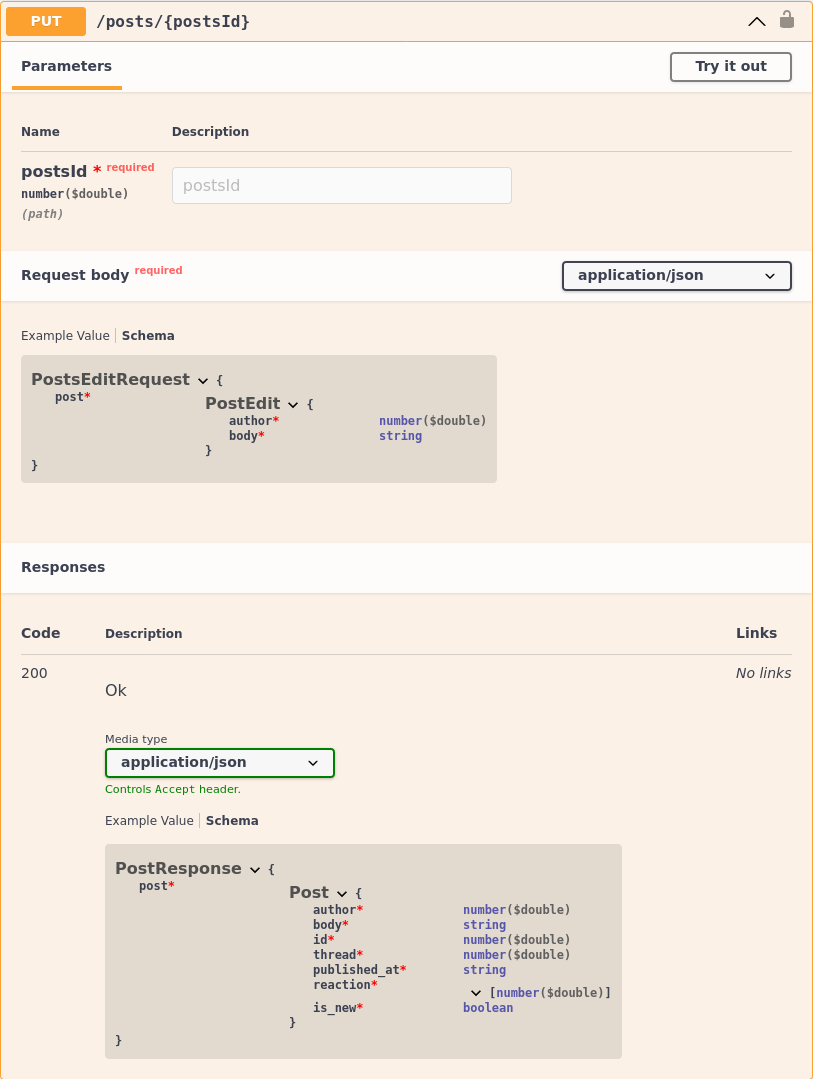
\includegraphics[width=\textwidth]{assets/img/swagger-ui}
\caption{The visualization of the post edit endpoint by Swagger UI}
\label{fig:swagger-ui}
\end{figure}

\mdstart

After the `swagger.json` definition file is generated on the backend, the `swagger-codegen`~[@swagger-codegen] tool can be used to generate respective code on the frontend:

~~~ JavaScript
public postsEditSingle(body: PostsEditRequest, postsId: number): Observable<PostResponse>;
~~~

Internally, this function will take care of handling authorization and possible exceptions, so that the developer can use this as a normal function, without the need to worry about its inner workings.

### Possible drawbacks

Because the definition of the API is stored within a separate project, this could in the future lead to a de-synchronization between the definition of the API and the backend code itself. Though, this threat would be present in some form unless the `swagger.json` can be generated directly from the backend code. If no technology like OpenAPI was used, then the possible issue would move on the client may be updated with less frequency than backend. The separate project is a compromise, which minimizes the risk of de-synchronization by using a simple to use syntax for the backend developers and easy changes implementation by regenerating the code from the Swagger definition for the frontend developers.

## Docker container

The only public instance of the OSI backend is for the production environment. The second instance, created for testing purposes, is only available from inside of the faculty network, which makes it inappropriate for wide testing by all OSI organizers, given that not every organizer is also student of the FI. This makes the need for another backend instance obvious. Furthermore, being able to easily create multiple instances for local testing during development decreases a chance of a larger issues, because of their local scope.

The backend project itself has only a few external dependencies -- except for Python 3 environment, it needs a [`isolate`](https://github.com/ioi/isolate/) project executable for sandboxing untrusted participants code and a database to connect to. By selecting a base Docker image of Python 3 based on [Debian buster](https://hub.docker.com/_/python) it is possible to create an environment simmilar to the OSI production server. Almost every required modification to the backend project can be done directly inside the [Dockerfile](https://github.com/fi-ksi/web-backend/blob/master/.docker/Dockerfile), namely:

- because `isolate` is not available as a Debian package, it has to be compiled manually. The Dockerfile downloads the built version from my personal Debain package repository
- for easier manipulation with the database, an SQLite database file will be used instead of MariaDB server used on production. This decision has a few implications:
  - the SQLite database backend does not automatically convert data types, so some source code patches were needed to fix data types passed to the database
  - SQLite does not fully implement all SQL language features, for example `CURRENT_TIMESTAMP + INTERVAL 1 SECOND` needs to be replaced with `datetime("now", "+1 seconds")`
- the server needs to be accessible from the Docker container's IP address, not only from localhost
- `isolate` requires the `/etc/` directory to be bind mounted as `/opt/etc`, which is not possible inside a Docker container, unless the container is started in a privileged mode
- the default starting script, which launches the server as a background daemon, needs to be replaced with a different container entry point that stays in the foreground, which is useful for starting the container in an interactive mode

The data of the backend server, together with the SQLite database file, are kept externally and are only bind mounted to the container, so that rebuilding the docker image does not erase them. Only when the entrypoint of the container is executed the data is mounted into appropriate location. To prevent insufficient permission when accessing to the data by the unprivileged `ksi` user inside the container, the real owner is masked by using `bindfs` tool.

Because the container is running in a privileged mode with shared `/dev/fuse` for the `bindfs` tool, it is currently undesirable to execute production server inside the container, as it may pose a security risk. On the other hand, the container is fully suitable for usage during the development of the frontend application. Furthermore, the whole docker container can be packaged inside a `.tar` file and then transferred to another machine, making the process of creating another backend instance faster. This feature was used when deploying a temporary [testing server](https://ksi.ahlava.cz/api/years), which is available for all OSI organizers and is running inside the docker container.

\end{markdown*}

\mdchap{Selecting framework for a new web application}

Choosing the right framework, if any, largely impact the structure of the whole application. Because one of the main goals of this thesis is for it to be easily maintainable and quick to understand, the framework must be corresponding to these needs. Given the nature of the composition of the OSI organizers team, where most of the team members do have different skill sets, it is plausible that some of the next maintainers of the OSI web application will have only a basic knowledge about web development in general. Most of this general knowledge is likely to originate from the course PB138 Modern Markup Languages and Their Applications on the Faculty of Informatics Masaryk University. With that in mind, it is evident, that the selected framework needs to be fast to learn and easy to understand with as little background as possible.

## Developing without framework

Even though that it is possible to develop whole application without the use of any existing framework, this approach gains significant problems with the enlarging size of the application. Given that nearly every modern page consist at least of three components -- HTML file defining the elements, JavaScript file with functionality and CSS file used to style the look and placement of elements on the page, it would be possible to import JS and CSS files to different webpages to reuse code. However, this does not apply to HTML, which would have to be a separate file for every web page of the application, resulting in a large reuse of a code. It would be possible to implement a logic that would create complex HTML components from predefined source templates, but this approach would effectively create a new framework. This new framework would then suffer from additional issues like lack of external support and previously untested code.

## Developing with a framework

For reasons shown in the previous section, the development of a larger web application without a framework is not ideal. On the other hand, when a framework is used in the project and then later is the framework marked as obsolete, it can be a challenging task to continue with a maintenance of the project, perhaps best shown on the example of the current OSI web. To select the correct framework for a project, it is possible to investigate the most used ones as they are expected to be supported for a longer period of time. Stack Overflow, a company best known for its site for Q~\&~A regarding computer programming, publishes results of annual survey among developers. According to the 2020 survey~[@stackoverflow-survey] with 36~291 responses from professional developers, the most used web frameworks with at least 25\% of positive responses are jQuery~(43.3\%), React.js~(36.8\%), Angular~(26.5\%). These are the frameworks that I have considered for the new OSI web application.

### jQuery

The jQuery library~[@jquery] is not a full-featured web framework, instead it aims to make common tasks like event handling, animations and document manipulation simpler. As a simple presentation of its capabilities, consider following code with plain JavaScript and jQuery~[@jquery]:

~~~JavaScript
// JavaScript
document.querySelector('button.continue').innerHTML = "Next Step ...";
// jQuery
\$("button.continue").html("Next Step...");
~~~

For its supposed different use case, the jQuery fully lacks advanced features like abstract component creation and styles encapsulation.

### React.js

React~[@reactjs] is a web framework that is being taught on the PB138 Modern Markup Languages and Their Applications course on the Faculty of Informatics Masaryk University. It introduces its own syntax called JSX~[@reactjs-main-concepts]. JSX is a syntax extension of JavaScript, which allows writing HTML template together with JavaScript logic:

~~~JavaScript
function formatName(user) {
  return user.firstName + ' ' + user.lastName;
}
function getGreeting(user) {
  if (user) return <h1>Hello, {formatName(user)}!</h1>;
  else return <h1>Hello, Stranger.</h1>;
}
~~~

The practise of putting JavaSript code and HTML DOM together is useful for the understanding of code by eliminating the need to look on multiple places, possibly split between files. The way of organizing code parts is completely in the hands of the developer.

Main concepts of react are based upon creating components in a form of JavaScript function or ES6 class, which can then be used directly inside the JSX. Component-state management is implemented by saving the state locally and passing functions to child components, which can then propagate events by calling the passed functions as callback. This way of state management, especially when combined with components implemented as functions, makes it possible to produce a cleaner code with well visible dependencies.

The bare React.js without any dependencies does not contain additional features such as CSS encapsulation, meaning that any style defined and imported anywhere in the app will affect even parent components that match its selector, though this feature can be achieved by using the officially supported tool for creating React.js applications.

### Angular

According to the previously mentioned survey, Angular~[@angular] is a third most used web framework. Much like React.js, Angular allows creation of abstract components. Instead of creating the code structure manually, Angular provides a command-line tool `ng`, which handles common tasks, for example generation of code elements.

For faster development, the `ng` tool provides a sub-command `ng serve` which launches a web server presenting up-to-date version of the source code. When the source code of the application is modified, the web server automatically reloads the application without the need of developers interaction. However, this approach is not suitable for the production environment -- to prepare the application a sub-command `ng build` exists. This sub-command copies whole application code and assets into a sub-folder, replacing Angular-specific schematics with plain minimized JavaScript code. It also bundles multiple source code files together to lower the required number of requests to the web server from the client.

#### Long-term support

Angular publishes a new major release in a 6-months long cycle, while previous major releases will receive security patches for the next 12 moths, making an update necessary every 18 months~[@angular-releases]. To easy the process of updating between two version, Angular provides a [guide](https://update.angular.io/?l=2&v=12.0-13.0). The guide lets the developer choose the applications complexity and based upon that it will present the developer with a checklist of required steps to perform. For applications with medium complexity without a wide range of third party dependencies, such as this thesis, is applying the update to the newer Angular matter of tens of minutes.

#### Component

Angular component~[@angular-component], generated by executing `ng generate component \%component-name\%`, consists of three files -- `.html` file describing elements that will be placed inside this component when used inside DOM, `.scss` file for styling said HTML file and `.ts` file describing functions and code logic with the TypeScript language. Unlike React.js, Angular uses styles encapsulation by default, so that styles defined in one element do not interfere with styles from other elements. This allows for using shorter CSS class names, whereas without encapsulation, it would lead to collisions with other elements without specifying any prefix. It is possible for the `.html` file to reference variables and methods declared in the `.ts` code file - they can be used to display values, perform logic operations or loops or for passing data to children components. The methods can be used as a handler for events from user or from other components, or their return value can be used same as a variable.

When a value of a variable changes, the new value is reflected also to its template by recomputing a re-rendering it. Because this operation can be computationally difficult, it is possible to change the change detection behaviour to only update when requested from a code. Angular also provides a so-called two-way data binding, which, when a variable is assigned to an `<input>` HTML element, synchronizes the value of the variable with the value of the user input. Though, both these concepts can be improved with reactive development style, they provide an easy to understand baseline.

#### Services

A service in Angular~[@angular-service] is a code structure, that can be injected into a component or other components. It can be generated by running `ng generate service \%service-name\%`. In its bare form, the service serves a purpose of sharing a code logic between multiple components. With default setting kept, only up to one instance of every defined service is created that is then shared by all component referencing to it.

#### Modules

Every Angular component needs to be declared inside an Angular module. This declaration specifies the real location of the component after the project is built, having components from different modules in different files. This feature is best exampled when used together with so called "lazy-loading"~[@angular-lazy-modules]. By default, all modules are loaded as soon as they are available to the connected client for download. On the other hand, when the module is marked for lazy-loading, it is downloaded only when requested by the client. This approach saves bandwidth, as the client does not always need all components of the applications -- for example normal user does not need to load administrative interfaces.


#### Routing

Because build an Angular project creates a single-page application~[@spa], it produces only a single web document. Without any additional implementation of the navigation, the application would be limited to a single path. The Angular provides a routing implementation as one of its core features~[@angular-routing]. With it the navigation is done by assigning an Angular component for a given route path. This component will be then displayed when user enters assigned path. This approach frequently needs additional cooperation from the web server from which it is server, as the server would presumably end with a `File not found` status code, because the requested path does not exist in the folder structure. This can be overcamed by instructing the web server to return the main file of the build Angular application every time it does not find requested path on the disc.


#### Reactive development

Even though not a direct part of Angular project, but rather its dependency is a RxJS library. Much like `Promise` in JavaScript, the RxJS library contains a class called `Observable`, which is based upon asynchronously executed code~[@learnRxJS]. Unlike `Promise` from JavaScript, the asynchronous code is not execute immediately after creation of the object, but rather only on demand. The second main difference between `Promise` and `Observable` is that the `Observable` can return value multiple times, the `Promise` only once. Because of the direct support of the RxJS library inside Angular, it is possible to assign an `Observable` directly inside component's template. The main advantage of this approach is that this can greatly improve performance by requiring re-computation and re-rendering only of a affected template parts.

The RxJS library defines two main participants inside the flow of an `Observable` -- the *emitter*, who generates and event by providing a new values, and a *listener*, who wait for a new value to process it. One emitter can have multiple listeners. Also given the on-demand nature of the library, when an emitter has no listeners attached, the code logic of the Observable is newer executed. The emitted value can be also changed or filtered by using functions provided by the RxJS library.

To demonstrate the power of these features, consider following example: The user wants to login to a web application, so he fills username and password and then clicks on the login button. This click emits an event to an observable `loginSuccessful`, which will take the value of username and password and send them to the backend server. If the server approves sent credentials as valid, the `loginSuccessful` observable will emit a value of `true` and `false` otherwise. A listener called `menuContent` waits for an emission of a new state from the `loginSuccessful` observable and then transforms the content of menu on web page based upon new state, requiring re-rendering of only a small portion of the whole page. Second listeners listens only for `true` emission from `loginSuccessful` by filtering emitted values and then shows a welcome dialog to a newly logged in user.

As seen from the example, even basic the chaining of events can reduce code complexity and duplication, while simultaneously increasing application speed.

\end{markdown*}


\mdchap{Final web application}

## Application architecture

\begin{figure}
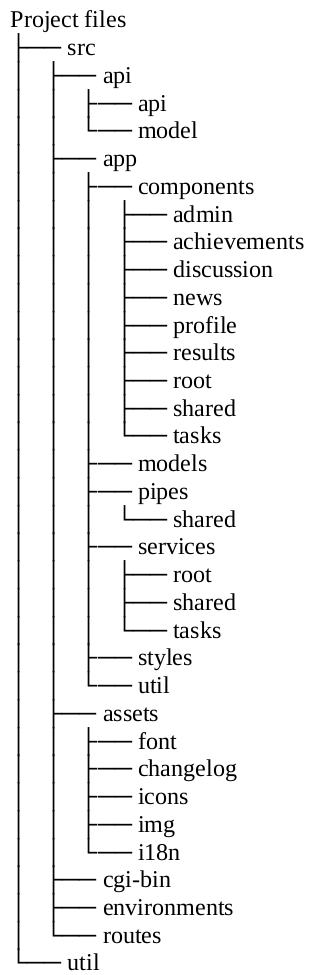
\includegraphics[width=.3\textwidth]{assets/img/file-tree}
\caption{The directory tree of the new web application project}
\label{fig:file-tree}
\end{figure}

### Project's directory tree

The project's file tree is a important architecture design choice as it will influence whole project. Because the Angular framework has a set directory structure~[@angular-tutorial], this projects expands upon it to make it as easily accessible to new developers as possible (\ref{fig:file-tree}). The project's root directory contains two main subdirectories -- `src` with the source code of the application and `util` for helper scripts that perform automatic tasks.

#### Source directory

Same as Angular defaults, the source directory contains `app` subdirectory for web application code, `assets` for holding static files that are not direct part of the code and `environments` that define constants specific for every instance (for example URL for the backend server). The `api` directory holds all code generated by the `swagger-codegen` tool (\autoref{chap:swagger-codegen}). Inside the `cgi-bin` directory is located the script required for automatic deployment (\autoref{chap:autodeploy}).

##### Application files structure

The application files are split into subdirectories based upon their Angular type (`component`, `model`, `pipe` and `service`). Next split is upon their module (`achievements`, `discussion`, `news`, `profile`, `results`, `root`, `tasks` and `shared`). The modules (except for module `shared`) are respective to their relative application path -- e. g. components that are inside `news` module will have a path starting with `/news/`. This splitting is done both for more rational file placement and faster loading times by utilizing lazy modules (\autoref{chap:faster}). The shared module contains items that are shared across multiple other modules, for example the loading spinner, which is included in almost every page. Models, services and pipes all contain in their root an `index.ts` file, which exports all their members from their subdirectories, for possible future easier refactoring.

The `styles` directory contains global variables to be imported in components, SCSS mixins for common style adjustments, color palette definition and theme variables (\autoref{chap:theming}). The color palette is generated as shades from [internal OSI colors](https://github.com/fi-ksi/grafika). To make color replacement for other projects derived from this thesis as simple as possible, almost no other colors are used in the entire application, with the only exception being colors retrieved from project's third party dependencies.

Lastly, inside the `util` are defined static utility classes that are not part of single Angular type, but still used in multiple of them. These utility classes handle tasks like rewriting an asset URL retrieved from backed for the current web application to the location of the same assets inside the new application.

#### Utilities directory
\label{chap:utils}

The project's root `util` subdirectory contains shell scripts for automatizing tasks. The PWA requires icon to be of exact size, while the new web applications uses an SVG icon, the `gen-icons.sh` script takes the main SVG icon and converts into multiple icons with fixed resolution for the PWA. The `gen-api.sh` script automatically downloads the correct version of `swagger-codegen` tool (\autoref{chap:swagger-codegen}) and executes it to generate API code inside the `src/api` directory. It also attempts to fix the code that was generated in a faulty way -- for example by correcting the type of recursive array and replacing incorrectly typed function for downloading file from the backend.

The `gen-scss-theme.sh` is further explained in \autoref{chap:theming}, `gen-changelog.sh` in \autoref{chap:changelog}. All utility scripts have their respective alias inside `package.json` file for convenience -- `npm run gen.icons`, `npm run gen.api`, `npm run gen.theme` and `npm run gen.changelog`. 

### Theming
\label{chap:theming}

The new web applications supports switching between so called light (\autoref{fig:light-mode}) and dark (\autoref{fig:dark-mode}) modes. Internally, the modes are implemented as CSS variables, which get overriden by adding a `theme-dark` class to the page's `body` element. All CSS variables are defined inside `src/app/styles/theme.scss` with the name of their main occurrence, though they are reused as much as possible, to minimize required changes for other projects derived from this thesis. The CSS are not to be used directly in other styles, rather they are used as an input for `gen-scss-theme` utility script (\autoref{chap:utils}), which wraps all CSS variables as SCSS variables at the end of the file. The main advantage of this approach is that if a variable was removed or renamed, then an error during compilation will be shown for a missing SCSS variable, instead of silently ignoring missing CSS variable.

\begin{figure}
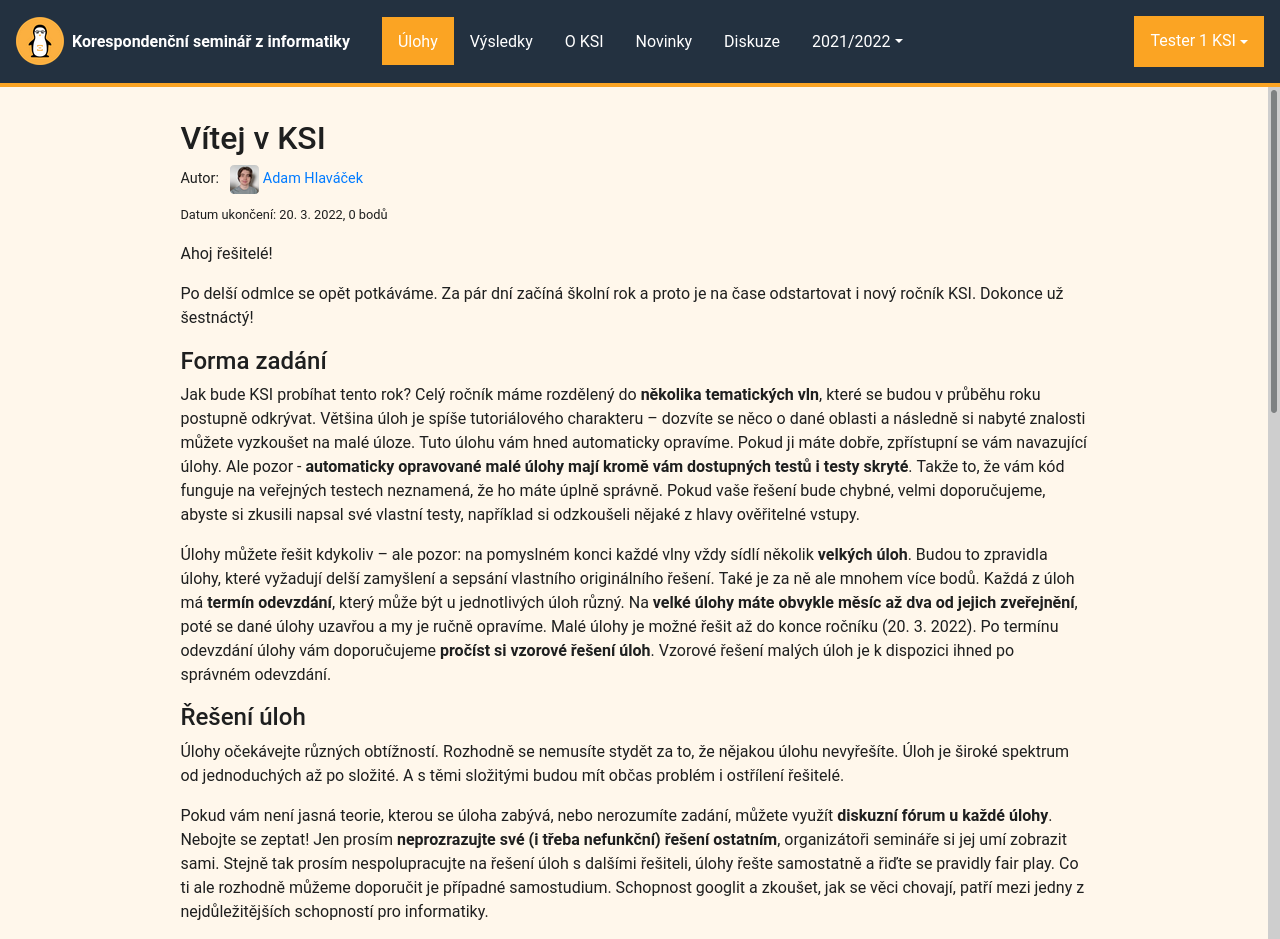
\includegraphics[width=.8\textwidth]{assets/img/light-mode}
\caption{Task page in a light mode}
\label{fig:light-mode}
\end{figure}

\begin{figure}
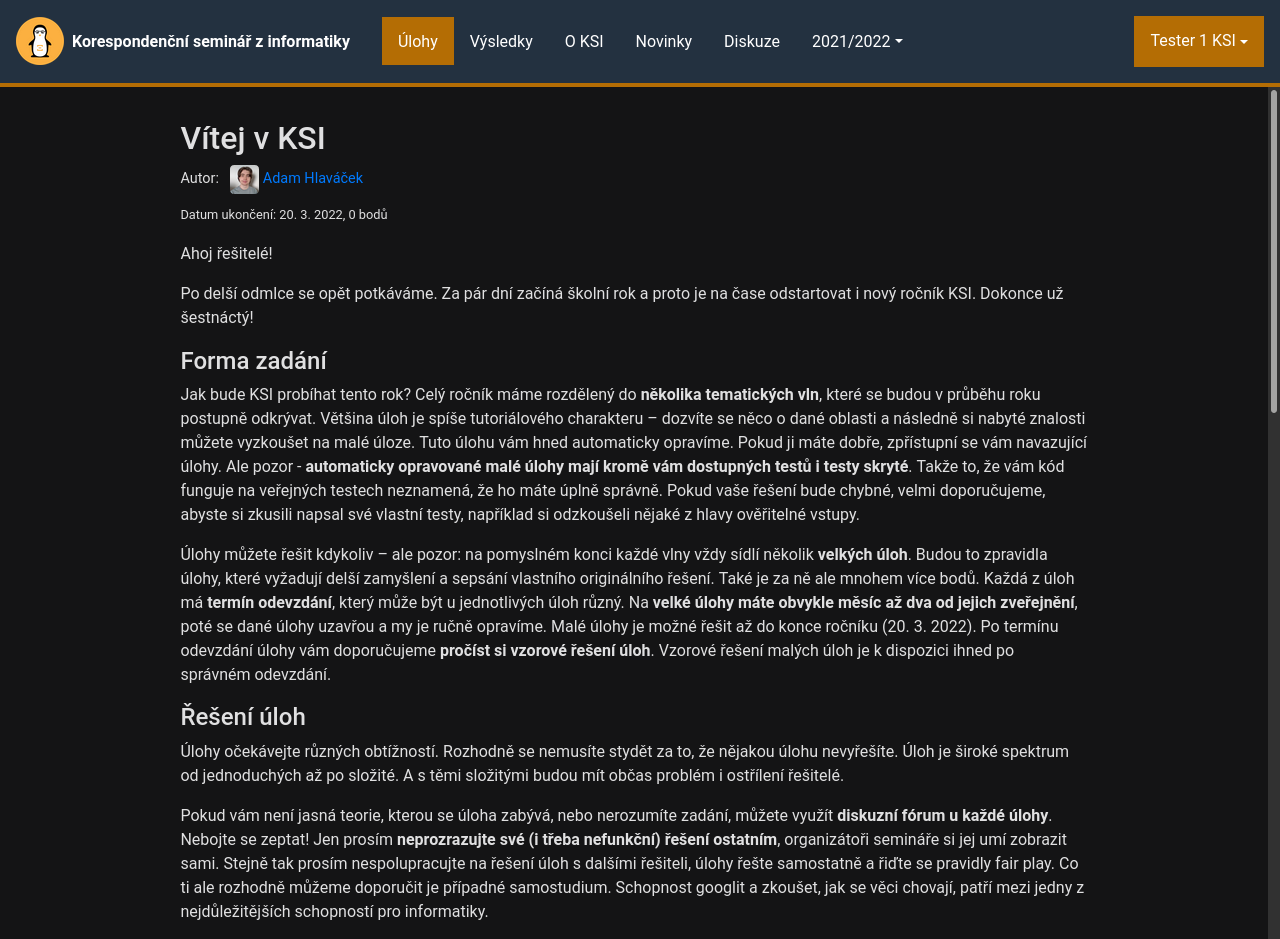
\includegraphics[width=.8\textwidth]{assets/img/dark-mode}
\caption{Task page in a dark mode}
\label{fig:dark-mode}
\end{figure}


### Translations
\label{chap:translations}

To make translations of this project or adjustments of texts for other project derived from this thesis, as simple as possible, almost all text strings are separated from the main code, the only exception to this rule being the page titled About OSI, which is expected to be full replaced with another page in other projects. The rest of the texts is placed inside a JSON file `assets/i18n/cs.json`. This file has a dictionary structure, in which are the string referenced by their qualified name -- for example, given the following `en.json` structure and Angular HTML component template

```JavaScript
// en.json
{
	"main-page": {
		"title": "Example title"
	}
}

// component template
<h1>{{'main-page.title'|translate}}</h1>
```

the result on the results page will be `<h1>Example title</h1>`. Also, by having all texts inside a JSON file, we are able to switch translations and target language by simply providing another JSON file during runtime of the application, as the `translate` pipe is implemented as a RxJS observable. Furthermore, because the qualified name format is used, it is possible to create gender-specific texts by appending e. g. `.male` or `.female` to the name, which is useful for Czech language.

In addition to translating the texts inside the application, the path names are also localized, however this localization is only applied during the build process of the application. The path names are defined inside the `src/routes` directory, where are files implementing `IRoutes` interface from project's models. Furthermore, by referencing routes through this interface rather than by path name, it is possible to rename application routes without multiple changes to application components.

### Automatic deployment
\label{chap:autodeploy}

When an process of automatic deployment is triggered the web application is automatically build and then released on selected instance, be it production, testing or other. The usage of automatic deployment lower the developer's work required to release the newest version of the application, because it takes care of repetitive steps and can be triggered for example by a simple push to a named git branch inside project's repository. The process can be also safer than manual deployment, because software tests can be a part of the automatic process. If some of the executed tests fails, the deployment can be rejected. This assures, that no version that does not pass the tests will be released to a production environment.

#### GitHub Actions

Because both current and web OSI web applications exists as project on GitHub, they can take advantage of the GitHub Actions feature. The GitHub Actions are a sequence of steps and commands that are to be executed in a virtual machine. They are defined as a YAML files inside project's `.github/workflows` subdirectory and can reference other projects as modules -- e. g. to create a new release of a GitHub project.

#### Current automatic deployment process

Currently, when a push actions is performed on one of watched branches, an automatic process is triggered. The process consists of building the web application and then copying the distribution files over SSH connection to student's home directory inside FI network. From there, the files are once again copied to the target server. The distribution files cannot be copied to the target server directly, because of security precautions from the FI which block SSH traffic to the OSI servers coming from outside the FI network. The main disadvantage of this process is that it requires an active student account. Also no tests are executed during the deployment process and a faulty code can result in a production downtime.

#### New deployment process

The new automatic deployment process is also triggered upon push to a watched branch. First, all requirements are installed and then the application is built for selected environment. During the build process, the code is checked for type safety and if any typing error is found, then the deployment is cancelled and the user, whose push has triggered the process, is notified about its failure. If the build process is successful, then a GitHub project release containing file `built.tar` with complete distribution files is created. The file `build.tar` has an unique address, which is passed to a deployment CGI script (`src/cgi-bin/dist-update.sh` inside the project's source tree) by calling it over HTTP. The notified CGI script then downloads the `build.tar` release and overwrites current files by the content of the `build.tar` package. A final step of the build process is to delete the created temporary release.

This new deployment process does not rely on any specific person to participate, only requirement is the existence of the called CGI script on the target server. To mitigate security concerns about downloading and untrusted `tar` file and blindly replacing own files with its content, the CGI script contains various methods of protection. Foremost, the script is supposed to be accessible only when a correct authorization is performed to the web server beforehand, which together with a strong password will mitigate most attack attempts, as those will be handled by the web server and the script will not be executed. If the attacker was to gain access by guessing the correct password, then the script itself will check that the owner and repository of the `build.tar` match with expected values and if not, refuses to perform the action. Finally, the CGI script is executed in a sandboxed environment with write access only to the distribution files, to prevent accidental file modification.

### Automatic changelog generation
\label{chap:changelog}

To keep the users of the web application informed about development progress, a changelog dialogue was shown whenever a change has been made since user's last visit (\ref{fig:changelog}). The changelog is generated automatically based on git commits history. This is possible due to respecting Conventional Commits specification~[@conventional-commits], where commits have a structure similar to `feat(category): description` or `fix(category): description`. Parsing such commit messages from git history is a trivial tasks, consequently making generating automatic changelog practically effortless. The changelog is generated on build time or by manually executing `util/gen-changelog.sh` script. Regenerating the changelog also updates application version number.

\begin{figure}
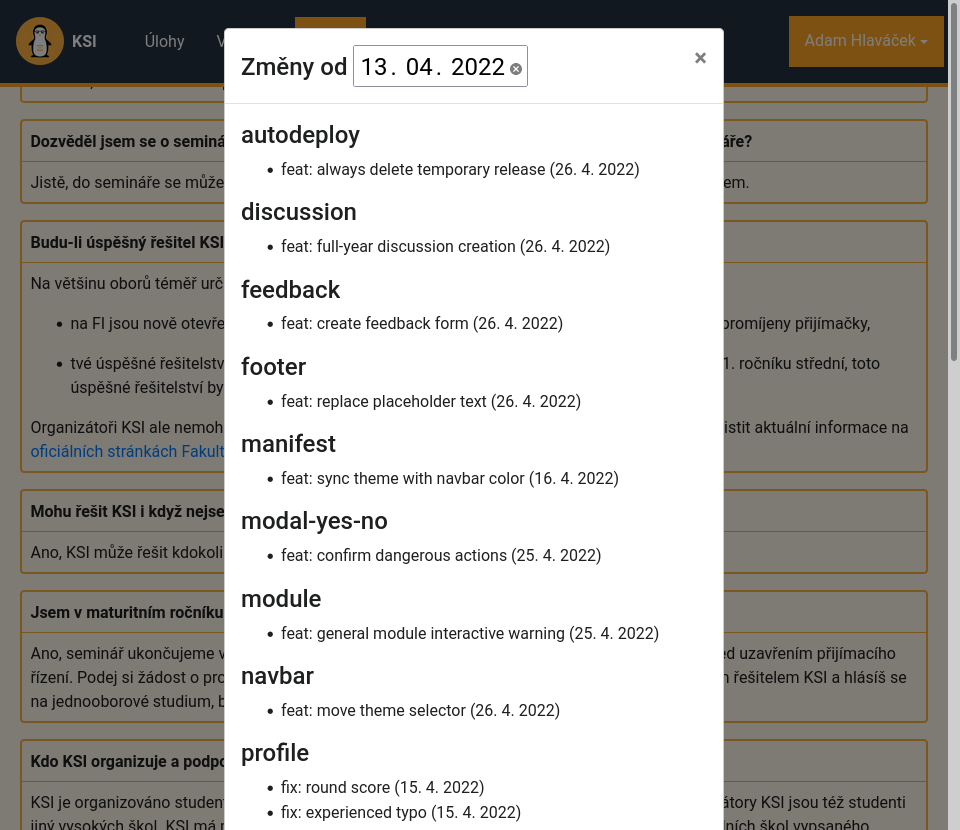
\includegraphics[width=\textwidth]{assets/img/changelog}
\caption{A changelog dialogue with recent changes}
\label{fig:changelog}
\end{figure}

### Login status and theme synchronization

Whenever user changes preferred colour theme or logs in or out, the information about this action is synchronized across all opened tabs through [`BroadcastChannel`](https://developer.mozilla.org/en-US/docs/Web/API/BroadcastChannel) API. This feature greatly improves UX in such cases when user opens multiple tasks that required log in at once without logging in. By simply entering his credentials in one of opened tabs, the status will be propagated across all tabs without any additional input from the user.

### Improved loading times
\label{chap:faster}

To improve loading times, all modules (except for `shared` module) are imported as Angular lazy modules~[@angular-lazy]. This assures that on the first load the application will load the minimal subset of code required to render content. Additional code from different modules is downloaded automatically when the user requests it, typically when navigating to another subpage. Furthermore, Angular provides a simple way to convert the application in a so-called Progressive Web Application, PWA for short. PWA relies on a Service worker technology, that works as a proxy for all network requests made by the application~[@angular-pwa]. As such, it can intercept the requests and instead of passing it through, return a version saved in cache. Most modern browsers support service workers, so the web application is cached automatically after first load. Subsequent call will be returned from cache, making loading pages instantaneous. On the background, the service worker checks if the code of the application was changed, then it is silently downloaded and applied upon next load of the application, making the transition between versions seamless. In the future, this behaviour could be a prerequisite for fully offline available OSI web application, though it would require backend modification and possibly break its compatibility with the current web application.

## UI Design

During the development of the application, I have followed following principles:

1. optimize the desktop page variant for displays of size 1920x1080
2. everything has to be accessible on mobile phone
3. provide an unique link whenever possible
4. prefer asynchronous operations
5. update smaller chunks of components instead of whole
6. cache mainly static but frequently accessed information

Because the design of the current still looks good enough nowadays, the overall look of the webpage is unchanged. The colour pattern was generated as shades defined from main OSI colours and all icons were reused from the current web application.

All text resources are either loaded directly from backend or from the `cs.json` resource file. This makes changing texts easier and also enables for easy translation to another language, as only a change of one file is required.

### Landing page

The landing page is referenced on every propagation media and as such is a first element of the OSI web application that possible participants will most likely see. The current landing page~( \ref{fig:welcome-curr}) uses a signification portion of space for large icons and long text blocks. It also presents a clickable button in the middle of an image, which is a disturbing design pattern. To address these issues, the new landing page~(\ref{fig:welcome-new}) splits the content into two rows so that newest information are visible without any scrolling required. The longer texts have been hidden behind carousel which is shown when the user clicks on one of the key OSI points in the middle of screen.

A second most notable design choice that differs from the current web application is the width and color of the navigation bar. In the current version, the navigation bar is located near the middle, whereas in the new application it covers full width of the screen with unified colours. This approach gives more breathable feel and is also easier to scale on different resolutions.

\begin{figure}
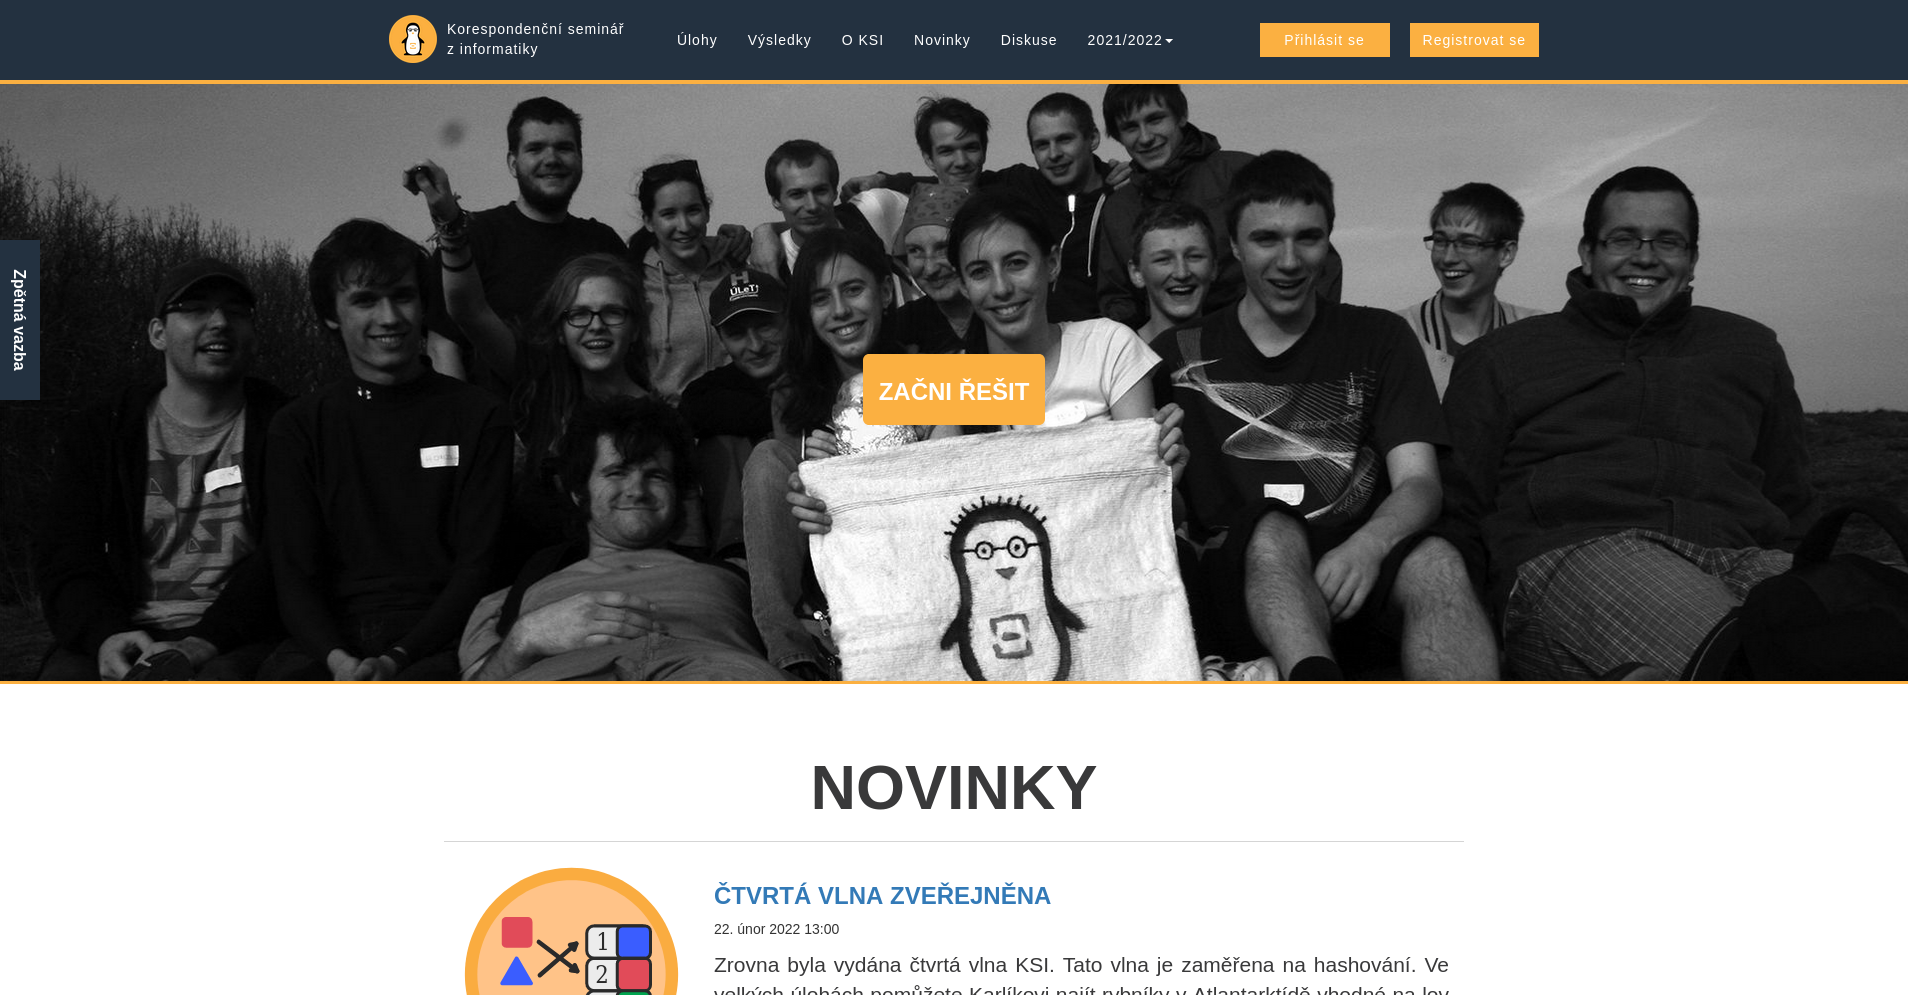
\includegraphics[width=\textwidth]{assets/img/welcome_curr}
\caption{The current OSI landing page on desktop}
\label{fig:welcome-curr}
\end{figure}

\begin{figure}
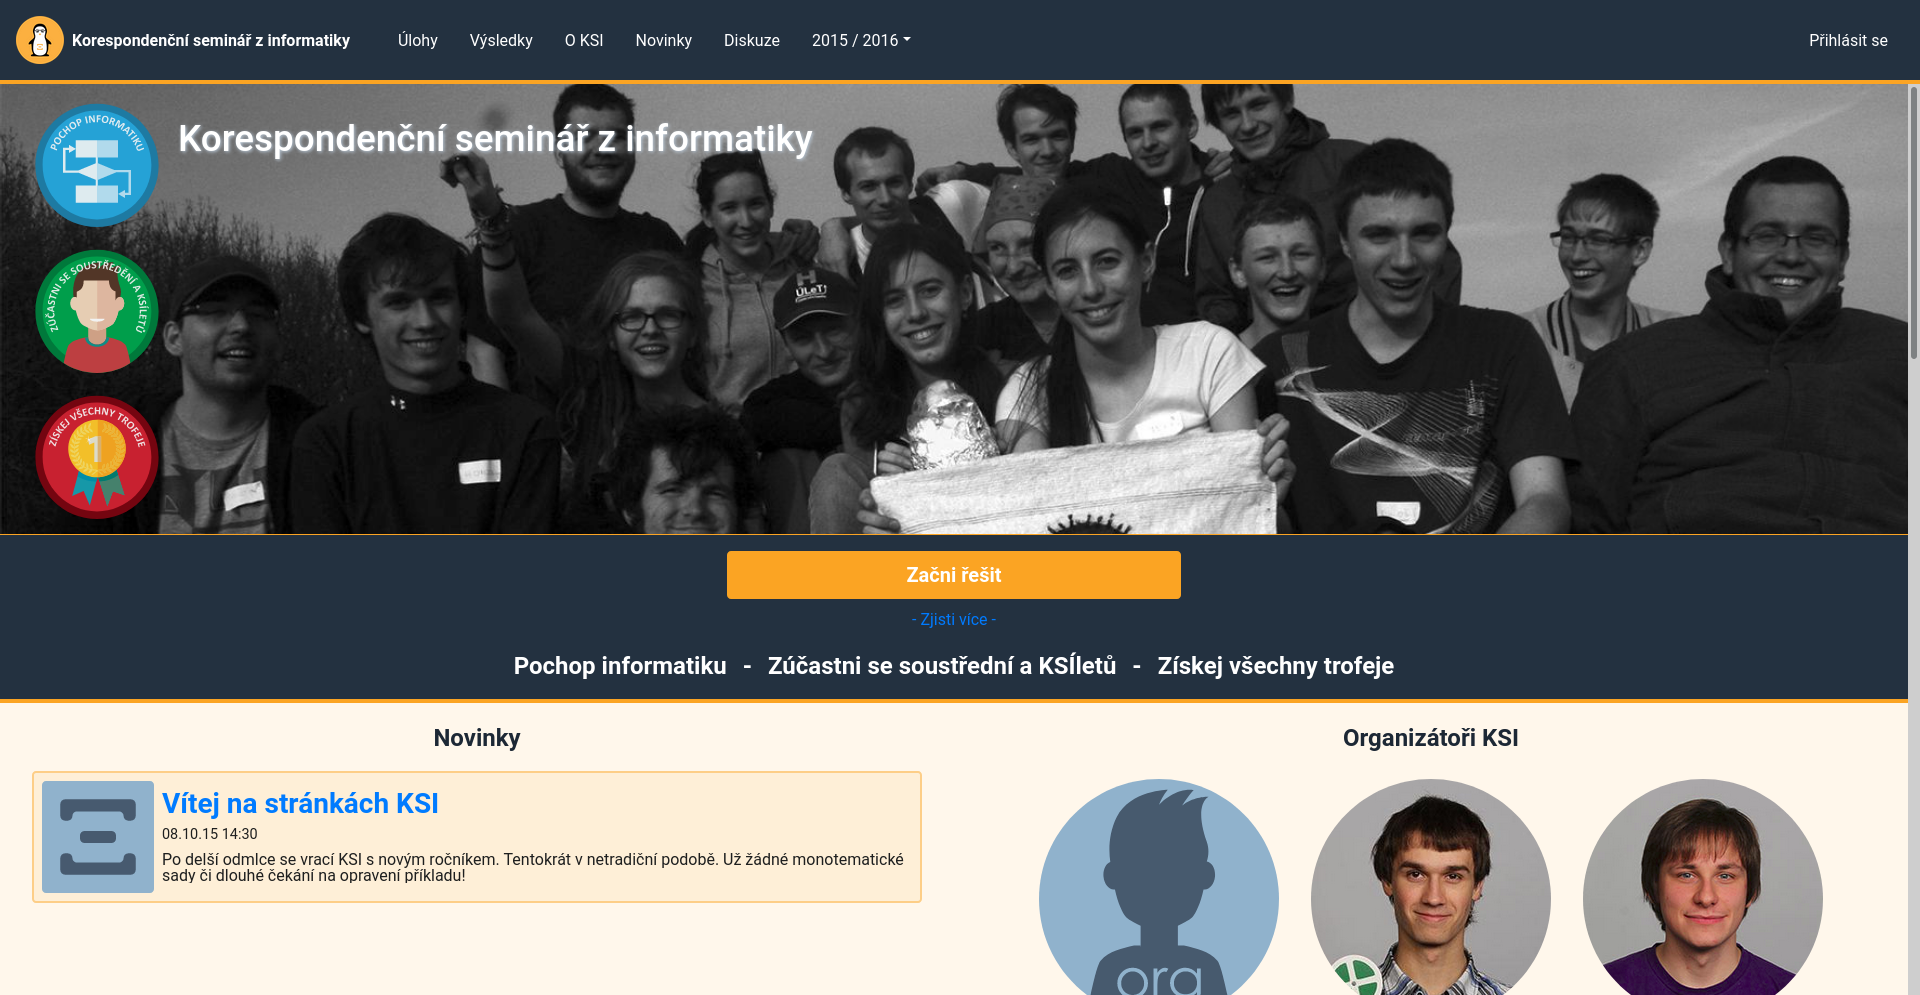
\includegraphics[width=\textwidth]{assets/img/welcome_new}
\caption{The new OSI landing page on desktop}
\label{fig:welcome-new}
\end{figure}

### Tasks graph page

The main point of OSI is a page with all tasks available to participants. The tasks are presented trough the form of acyclic graph, which can precisely represent which tasks are required to be completed before proceeding to the next ones.

The current version of the web frontend (\ref{fig:graph-curr}) shows a legend explaining the different graph node colors on the left, which moves whole graph slightly to the right side. Moreover, with a progress of a year, the graph could get more complicated and unclear. The new web frontend (\ref{fig:graph-new}) tries to take a maximum advantage of available page width. This is done by moving the legend into a modal dialog (\ref{fig:graph-new-settings}) accessible by a help button in the top right corner of the page. Given that the legend is mostly used by only new users of OSI web application, there is a little need to keep it visible all the time. Furthermore, to increase the clarity of the task graph, it is possible for the user to turn splitting the whole graph into multiple smaller graphs by grouping them into their thematic waves (\ref{fig:graph-split}). In this mode, the user can then keep open only the relevant parts of graph, presumably only the currently active OSI task wave.

Though, the most notable change can be seen when using the OSI web application on a mobile phone (\ref{fig:graph-mobile}). In the current version, the graph on the mobile is too narrow to fit, which results in multiple tasks overlapping. This makes it nearly impossible to open correct task. Instead, in the new web application, a special graph presentation mode was created. In this mode, the tasks are shown in the mode of a list, where tasks required to be completed before other tasks can be unlocked are shown first. This mode lacks information about different graph branches as seen on desktop version, but provides a viable compromise to usability on a mobile phone.

In the spirit of the third followed principle, all tasks in all modes are now rendered as HTML anchor points, instead of clickable canvas as in the current version. The advantage of this approach is that now every task can be searched by its name from within the web browser and multiple tasks can be opened in a new tab by pressing the middle button on the mouse.

\begin{figure}
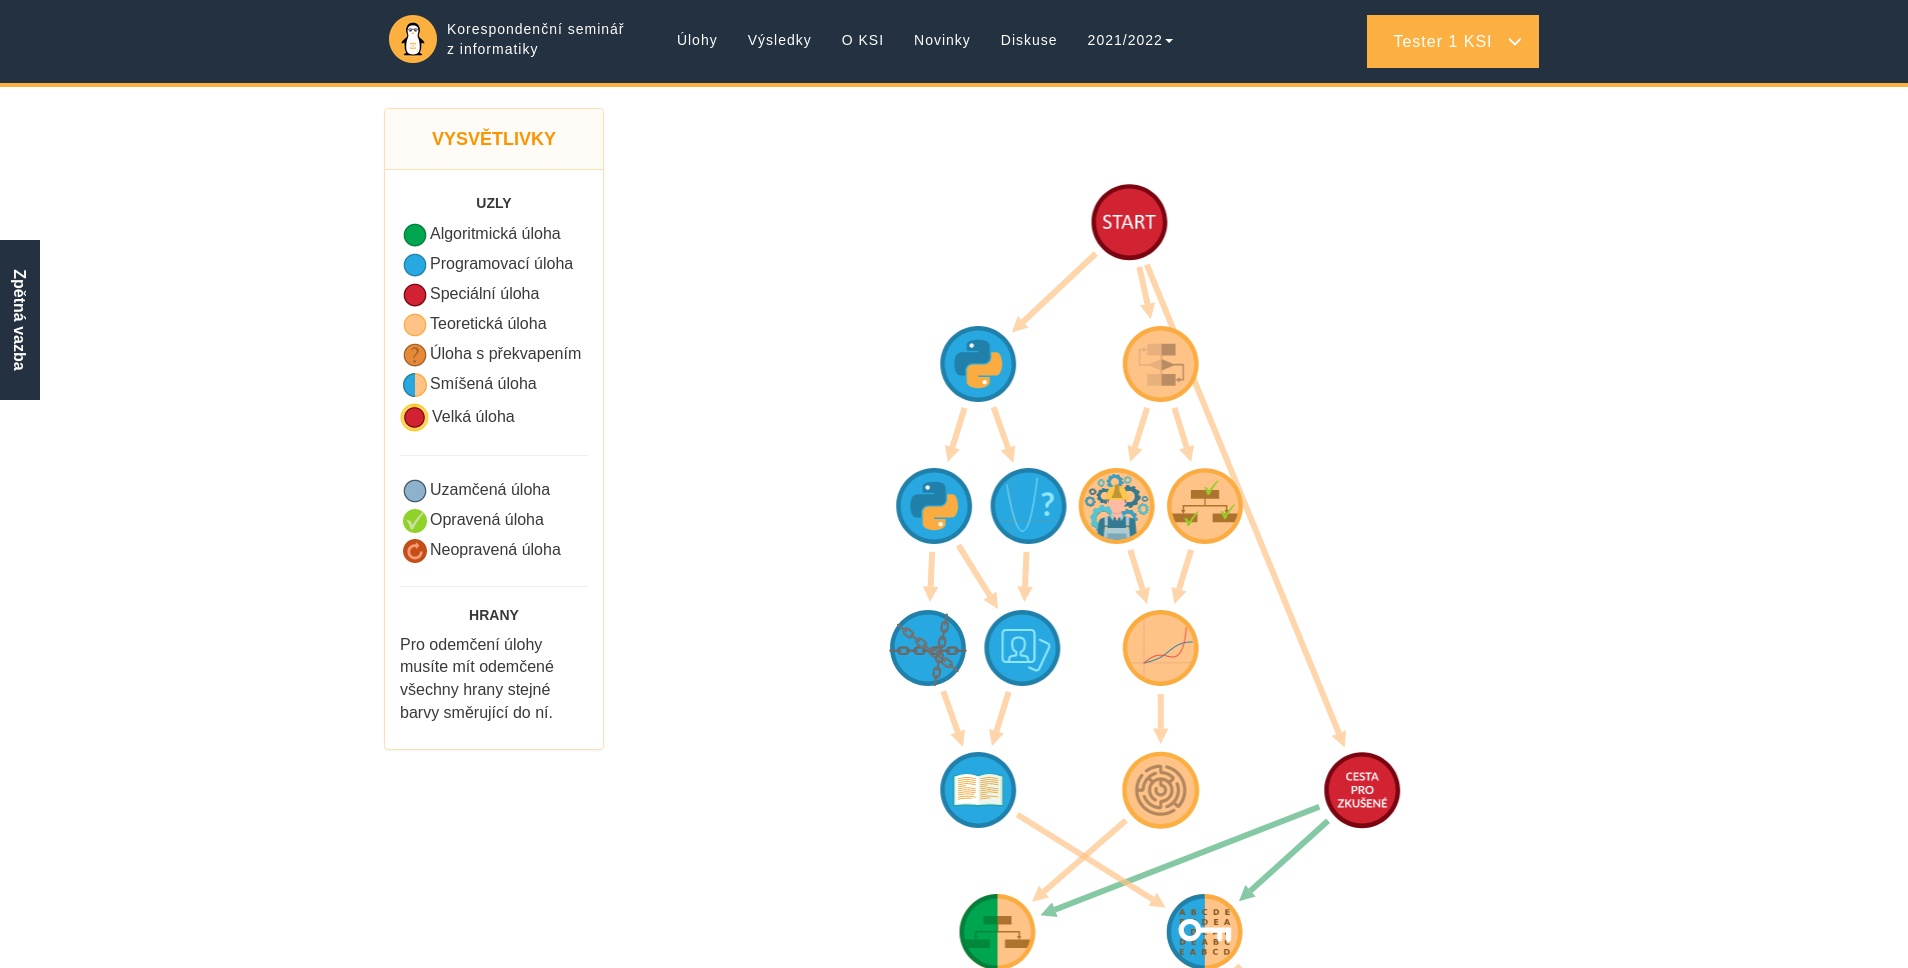
\includegraphics[width=\textwidth]{assets/img/graph_curr}
\caption{The current task graph}
\label{fig:graph-curr}
\end{figure}

\begin{figure}
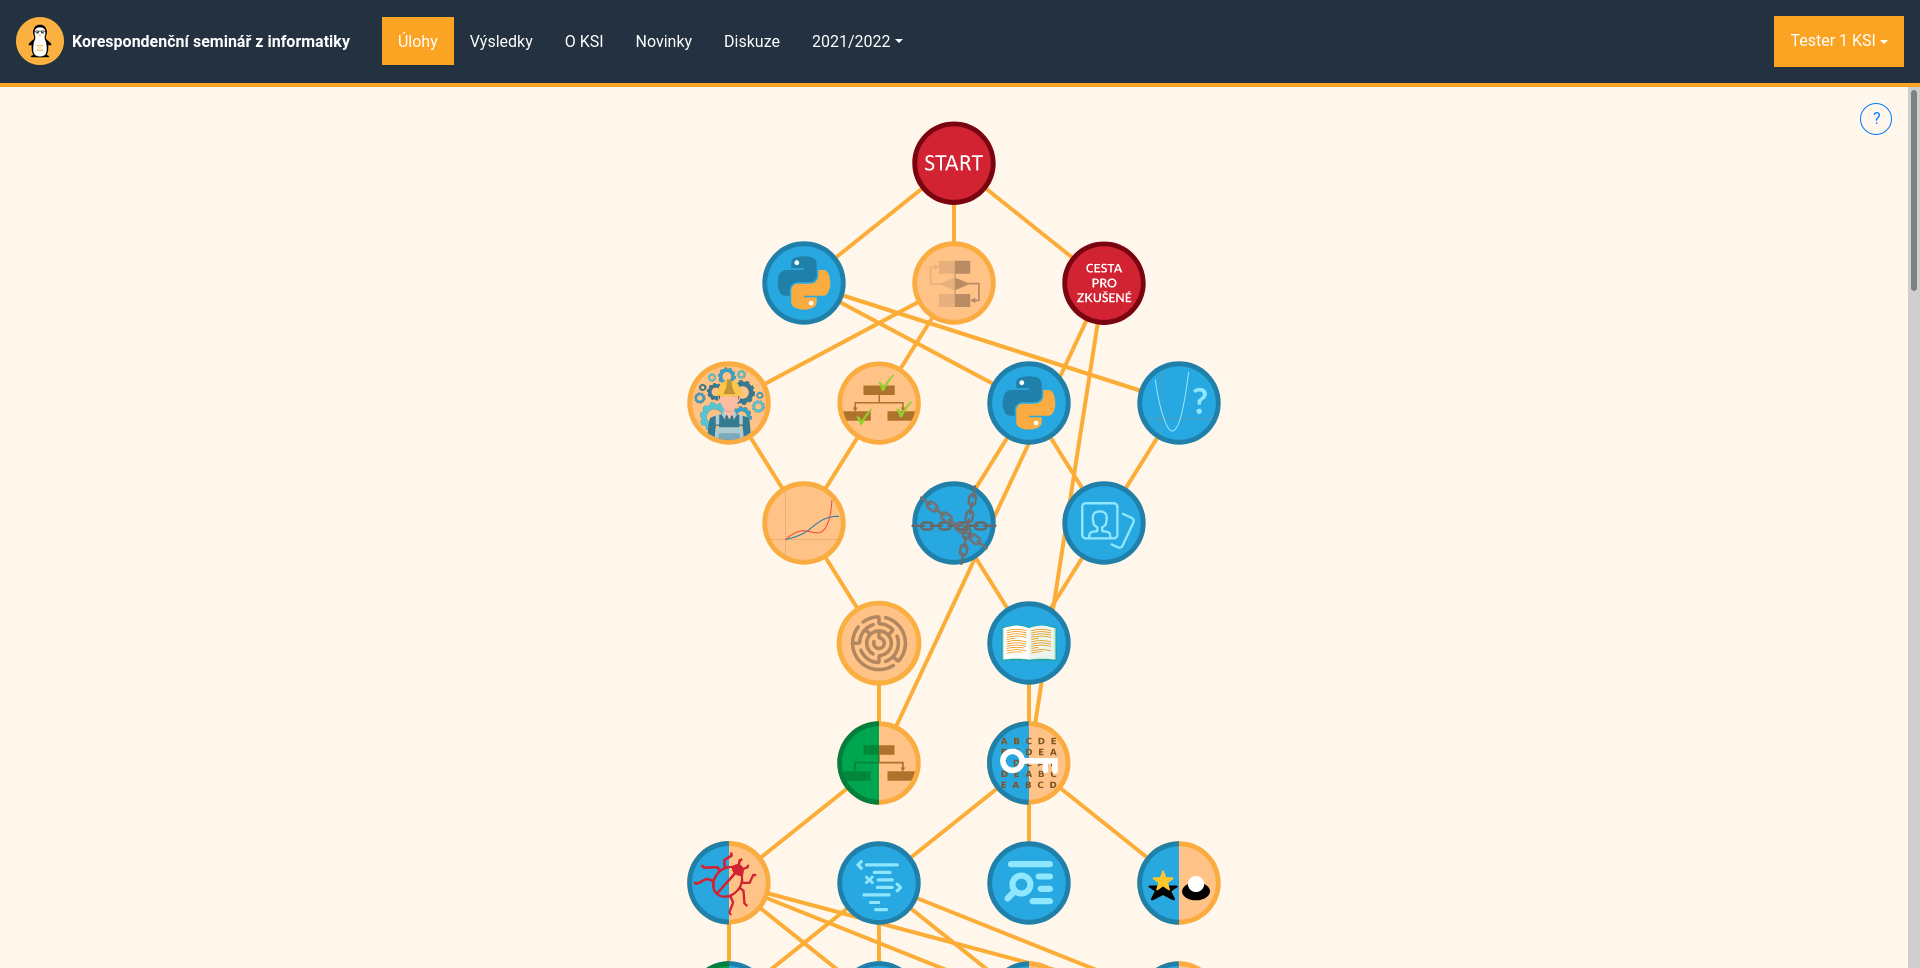
\includegraphics[width=\textwidth]{assets/img/graph_new}
\caption{The new task graph}
\label{fig:graph-new}
\end{figure}

\begin{figure}
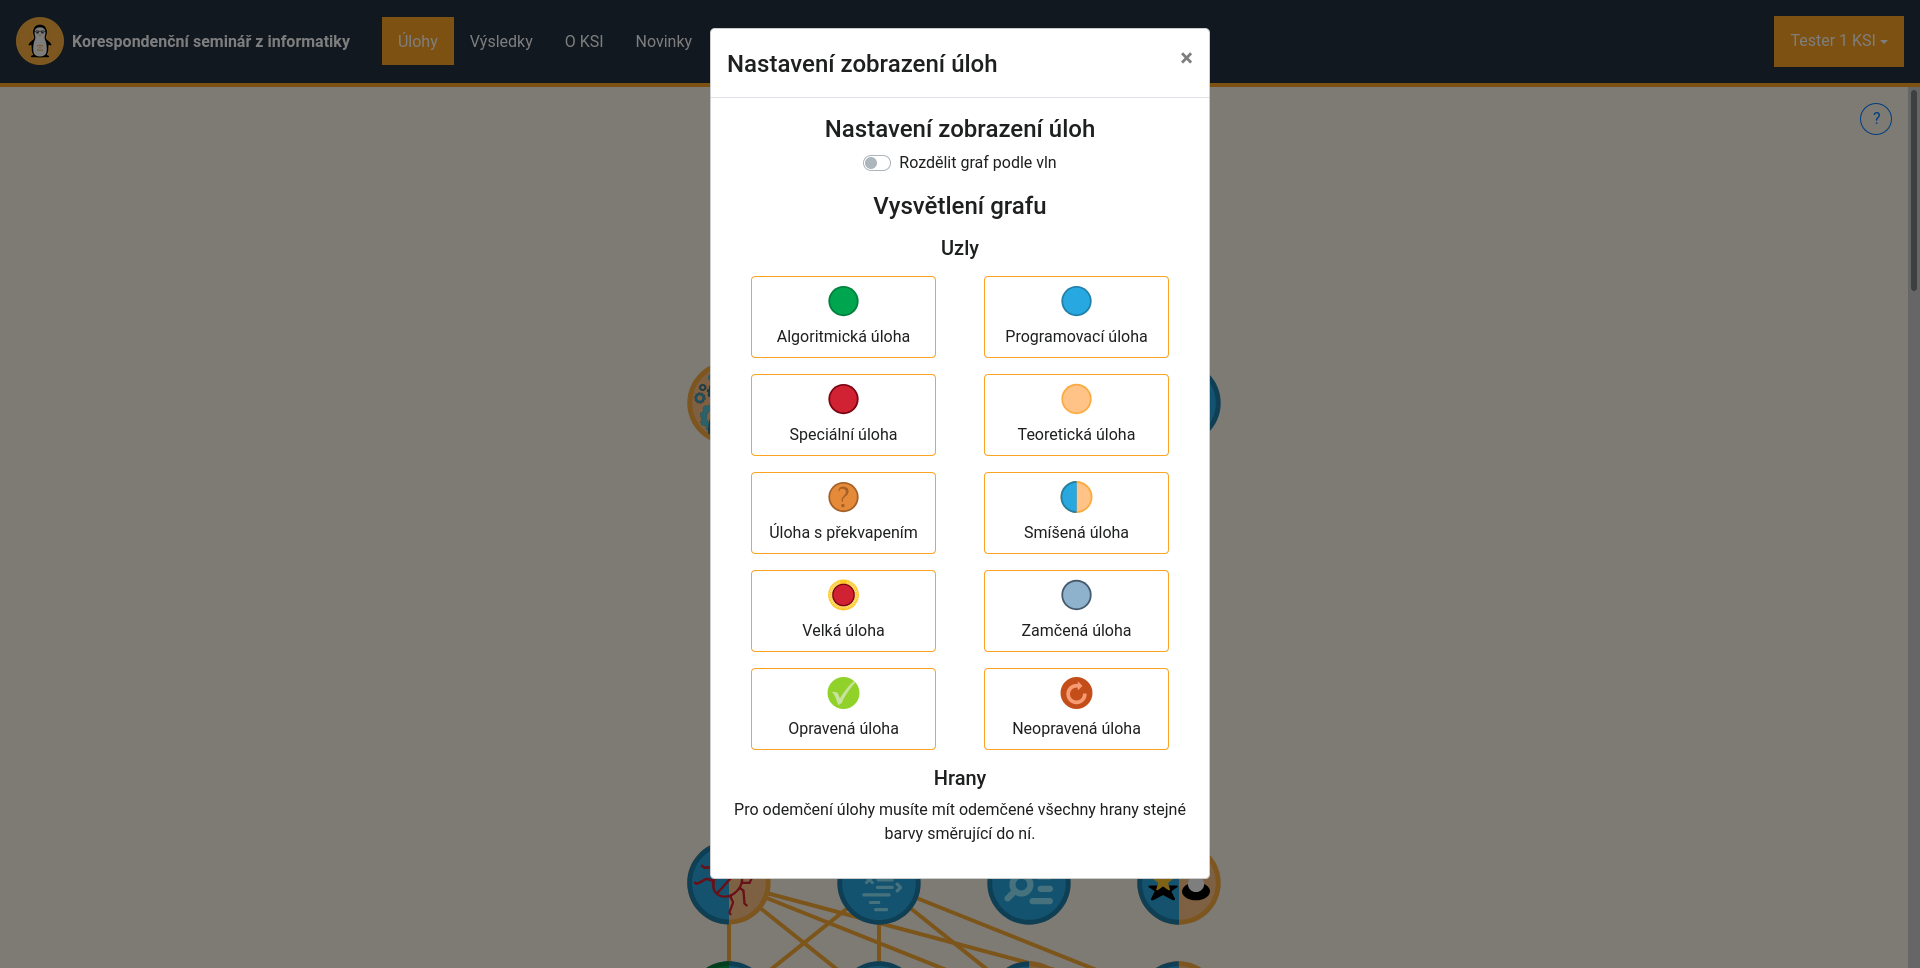
\includegraphics[width=\textwidth]{assets/img/graph_newsettings}
\caption{The settings of the new task graph with legend}
\label{fig:graph-new-settings}
\end{figure}

\begin{figure}
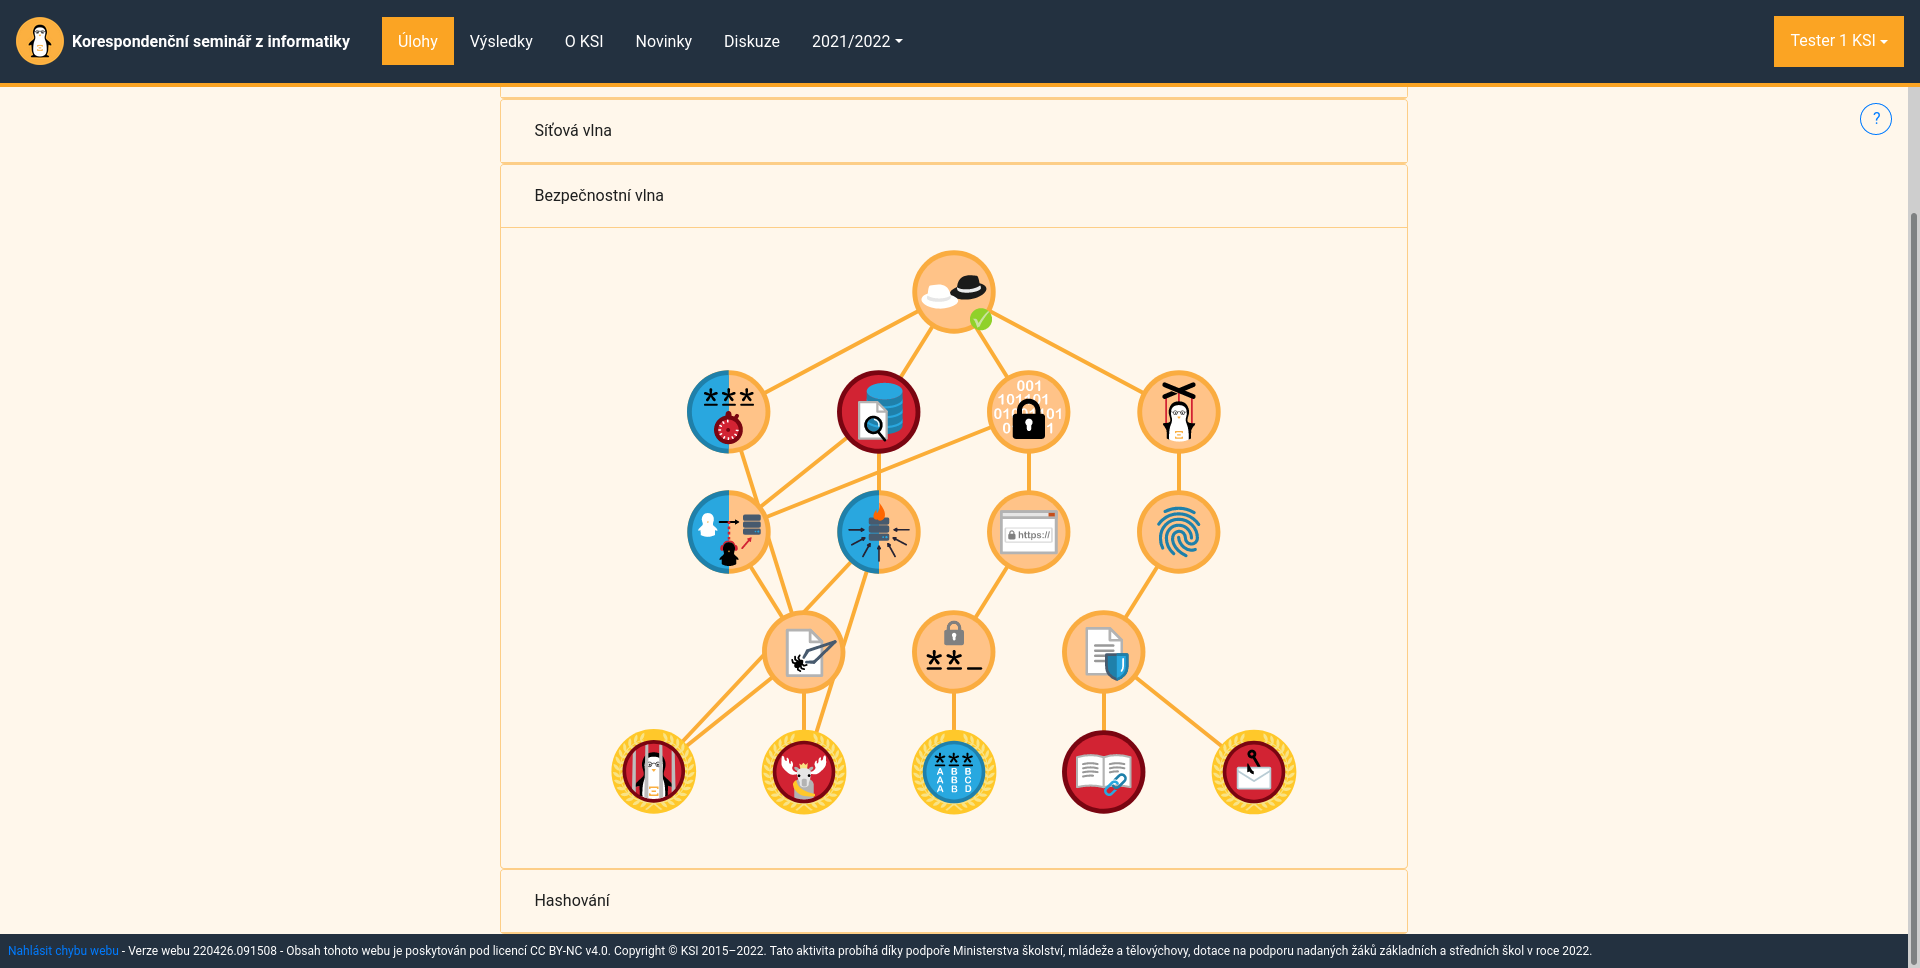
\includegraphics[width=\textwidth]{assets/img/graph_split}
\caption{The task graph when spitted by wave groups}
\label{fig:graph-split}
\end{figure}

\begin{figure}
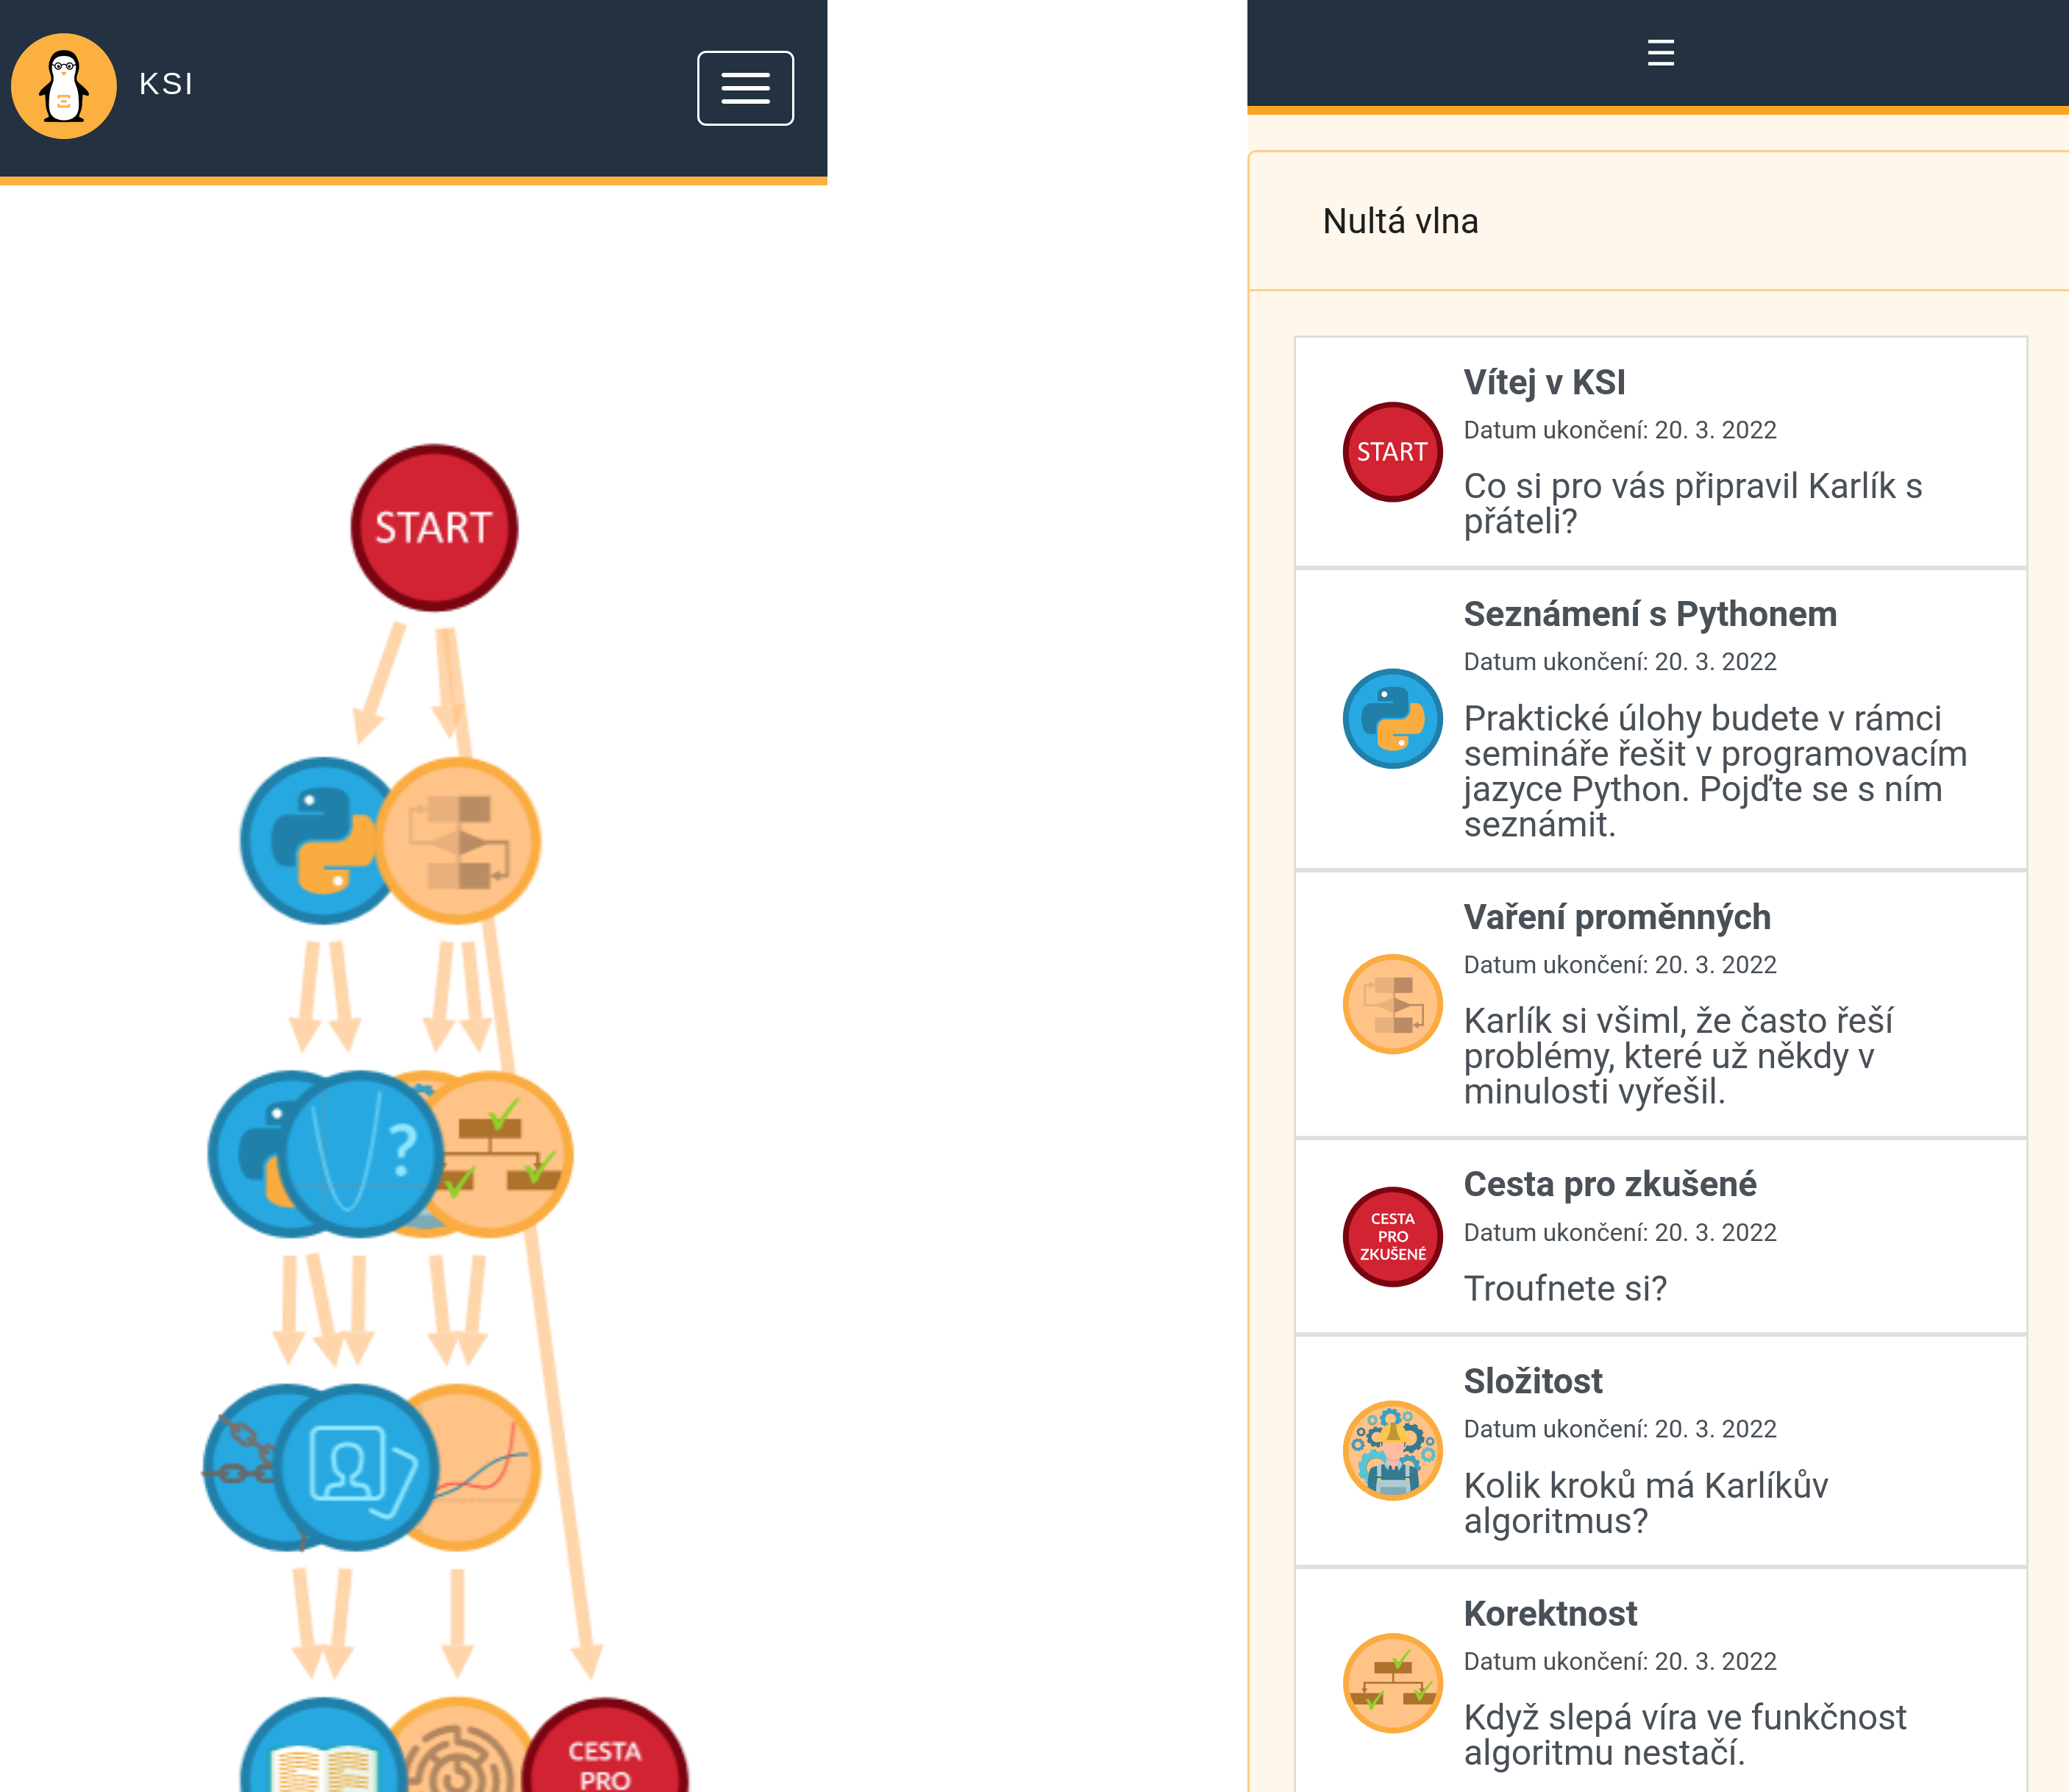
\includegraphics[width=.5\textwidth]{assets/img/graph-mobile}
\caption{The task graph when seen on a mobile phone (current left, new right)}
\label{fig:graph-mobile}
\end{figure}


### The task page

The functionality of a OSI task page remains almost unchanged, mainly a design modifications were made. In the current version (\ref{fig:task-curr}), the task has a section selection in its begging, where it may feel disruptive and complicated. Most of the time, the participant does not need to see discussion or his evaluation before he had read and tried to solved the task. The new web application puts all controls after the tasks assignment, imitating a style of an internet news article which has first title, then author, date of publication and then the content of the article. The content of the article is followed by a link to a discussion about said article. This design choice, together with less bright background, aims to lower possible distractions from the text of the assignment. Both discussion and solution are opened as a modal dialog on desktop to keep the page's scroll position intact. In the mobile version, where there is not enough space to open modal with more content, the assignment is replaced with requested section.


\begin{figure}
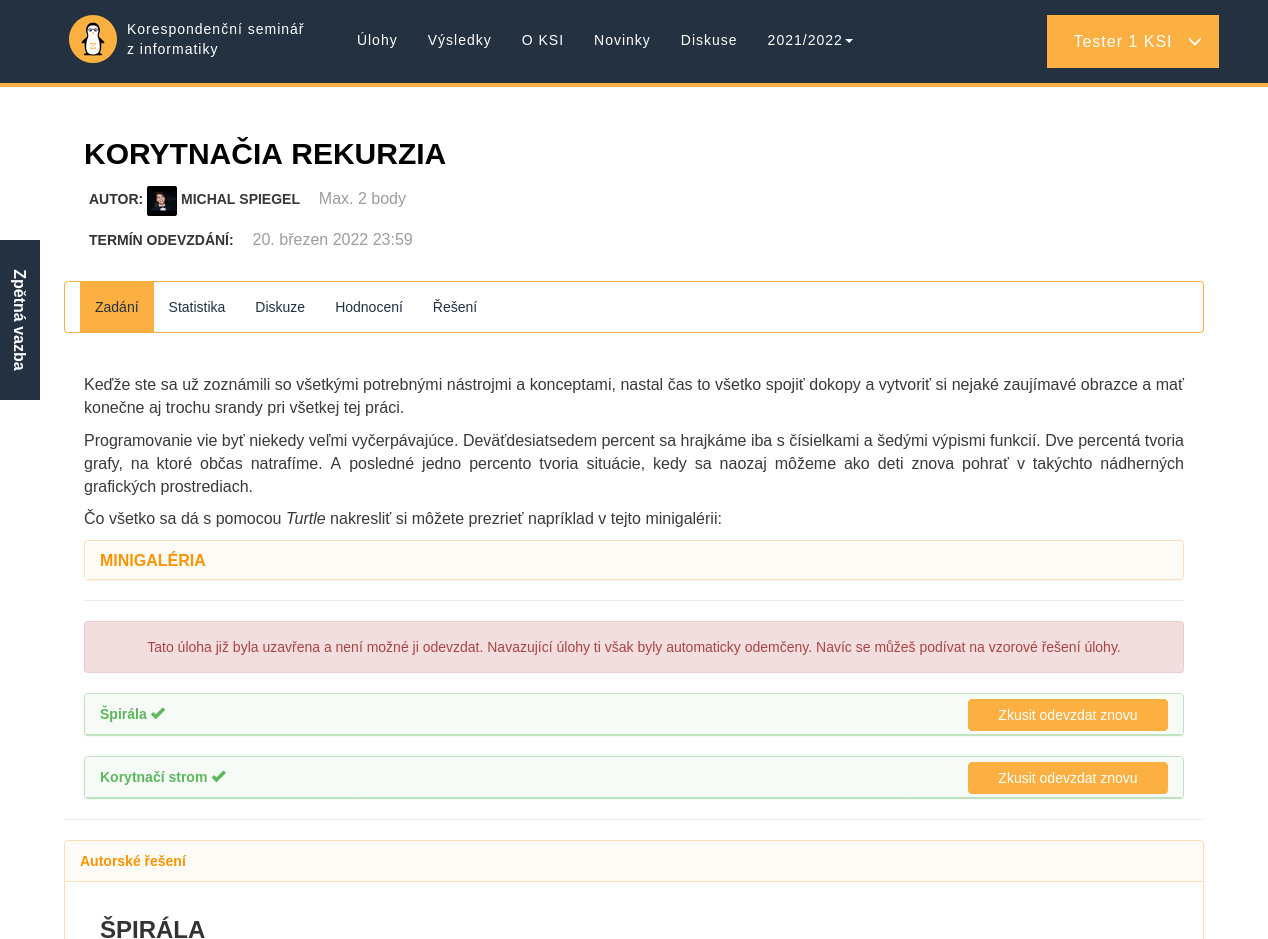
\includegraphics[width=.9\textwidth]{assets/img/task-curr}
\caption{The current look of a OSI task}
\label{fig:task-curr}
\end{figure}

\begin{figure}
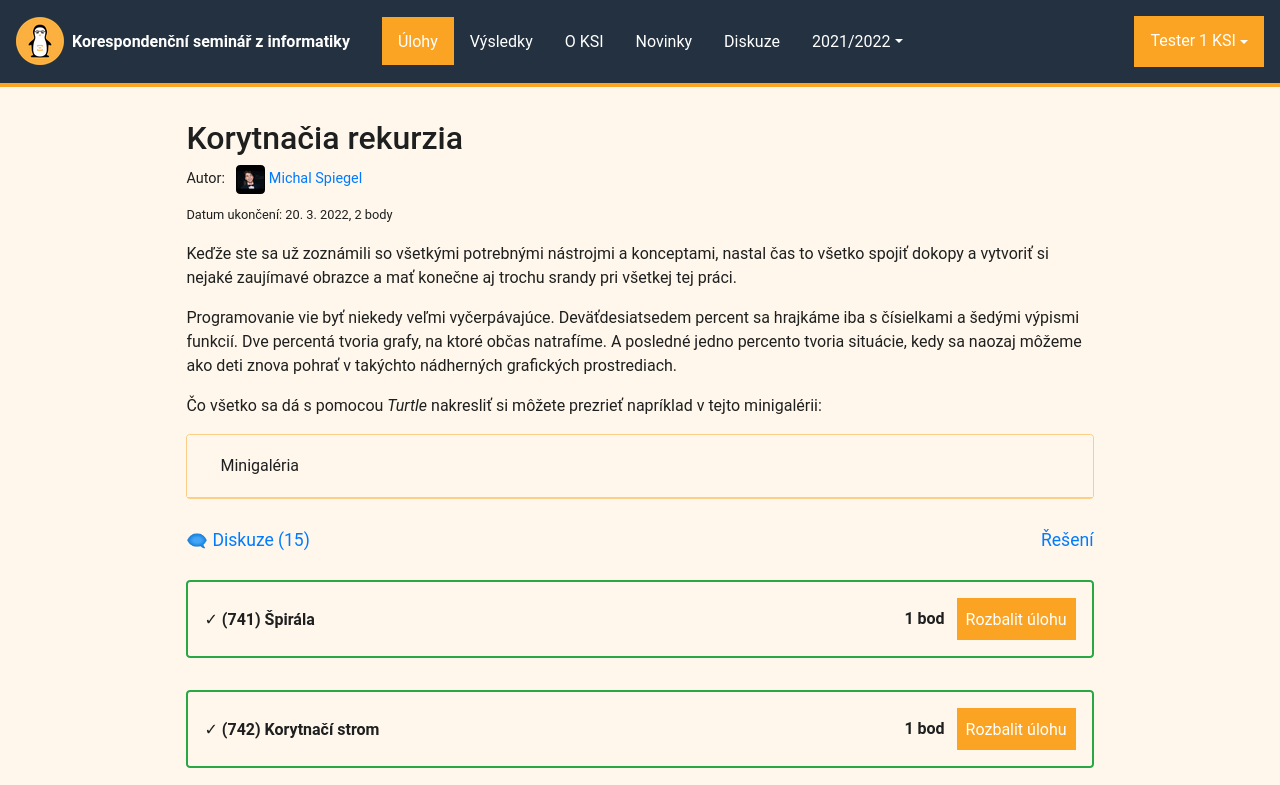
\includegraphics[width=\textwidth]{assets/img/task-new}
\caption{The new design of a OSI task}
\label{fig:task-new}
\end{figure}


### Discussion page

The discussion forum on OSI web consists of two pages -- first the selection of discussion subject thread and then posts within the tread.

#### Discussion selection

The selection takes form of a table with a name of thread and its posts count. The most notable difference between the current (\ref{fig:discussroot-curr}) and new (\ref{fig:discussroot-new}) design is that the current version contains a third column with a count of unread posts inside the thread. This columns is always visible, even if all posts had been read. Moreover, it shows white text on orange background, which may be difficult to read. In the new design, the count of the unread posts is shown only if there are any and is shown as a bold text in the post count column, making it easier for quick navigation.

\begin{figure}
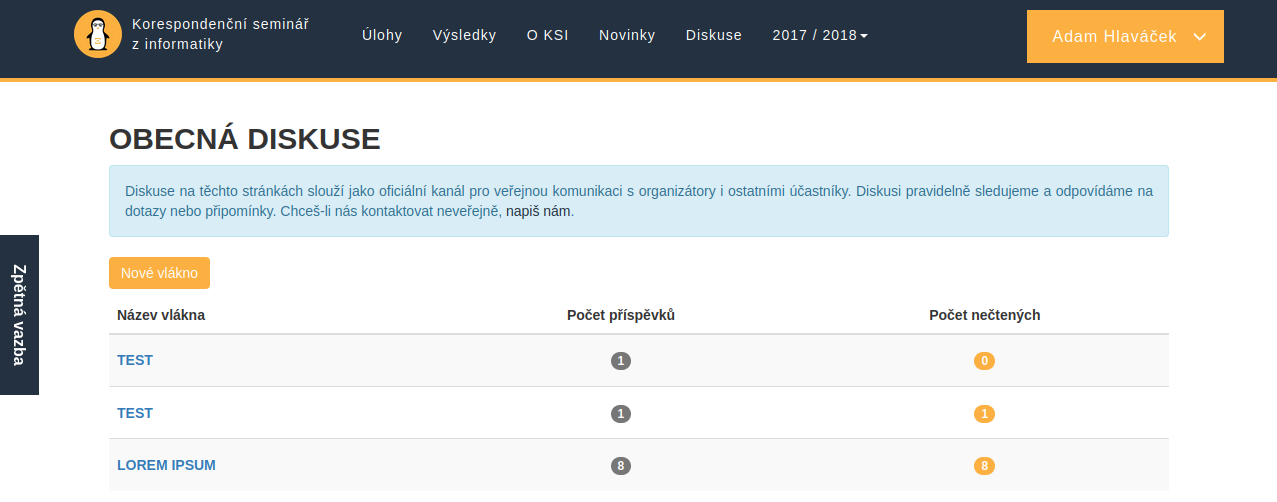
\includegraphics[width=\textwidth]{assets/img/discussionroot-curr}
\caption{The current look of a OSI discussion selection page}
\label{fig:discussroot-curr}
\end{figure}

\begin{figure}
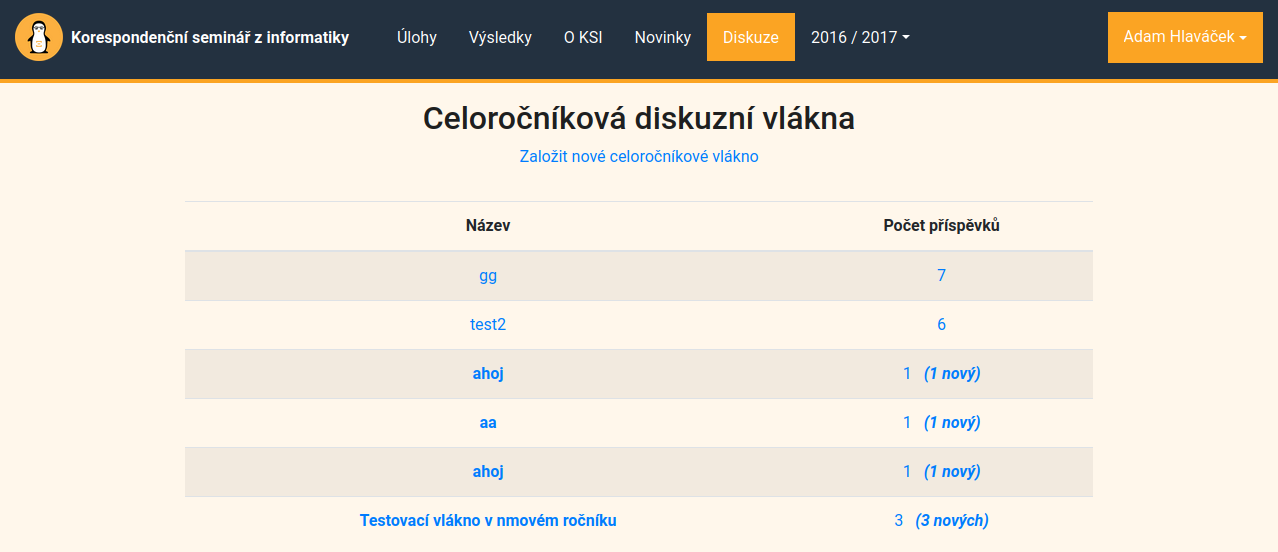
\includegraphics[width=\textwidth]{assets/img/discussionroot-new}
\caption{The new design of a OSI discussion selection page}
\label{fig:discussroot-new}
\end{figure}

#### Discussion posts

In the current version (\ref{fig:discuss-curr}), the posts have no borders and responses to a previous post are differentiated by a larger offset. However, if the posts receives multiple replies, it may overflow the maximum offset, which makes identifying which posts responds to which a difficult task. The new design of the web applications addresses these issues by adding borders to posts and a rails that indicate which post is parent of which reply. If the level of replies is too deep, then an additional button to unpack and continue within the reply thread is shown. When a reply thread is unpacked, it becomes the topmost post, hiding every post with a lesser level. By preternaturally unpacking replies, the web application assures that the structure of posts will never overflow maximum offset and as such will always be easily readable. A new added feature is an unique link to each post, which makes it easier to share it more precisely, rather than having to share the whole discussion thread and then manually search for the post content.

\begin{figure}
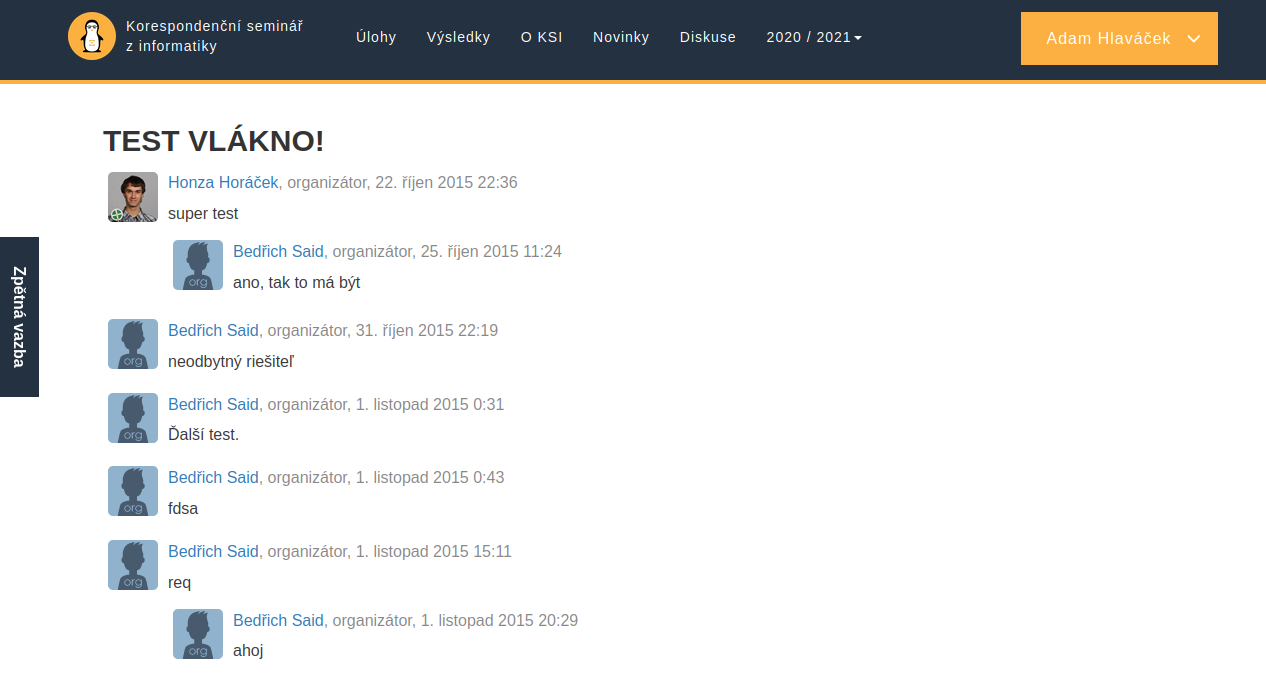
\includegraphics[width=\textwidth]{assets/img/discussion-curr}
\caption{The current look of a OSI discussion posts}
\label{fig:discuss-curr}
\end{figure}

\begin{figure}
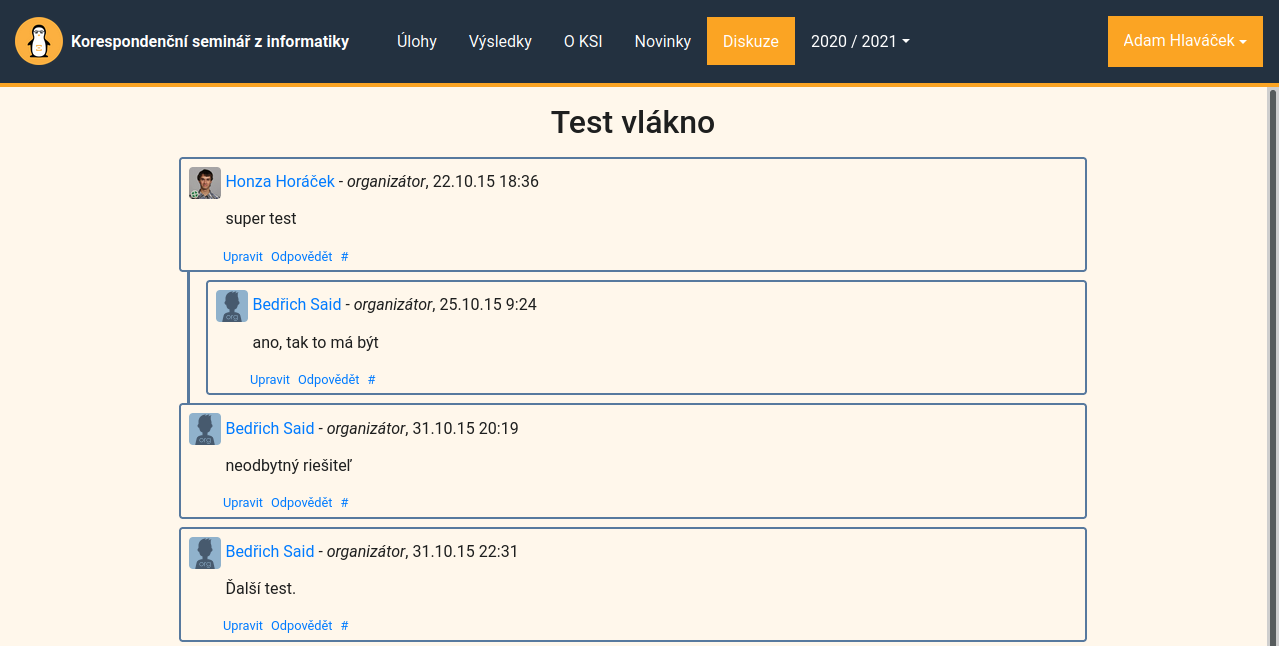
\includegraphics[width=\textwidth]{assets/img/discussion-new}
\caption{The new design of a OSI discussion posts}
\label{fig:discuss-new}
\end{figure}

## The second instance

During the spring semester 2022, the OSI organizer team was contacted by representative of the FI MU about creating a new online seminar for the newly accepted students with same basic structure as OSI. Participants will procedurally solve tasks about various subjects related to the informatics field and the environment of the university in general. Because the new web application was development with modularity in mind, it was selected as a main frontend for the new online seminar. The main tasks were changing used color pallet from OSI's to the one used by official FI MU website and rewriting occurences of OSI to the name of the new seminar, together with renaming affected path names. Because all these information are kept in separated files, which are then referenced, the process of modifying the values to desired outcome is not a time consuming process. Furthermore, following updates applied to the parent project can be applied to the [second instalment](https://github.com/fi-naskoc/web-frontend-angular) as well, by simply rebasing the patch commits on top of the new main branch of the parent project. The new online seminar, called [Jump-start the FI](https://naskoc.fi.muni.cz/), is set to begin at the end of May 2022.

\begin{figure}
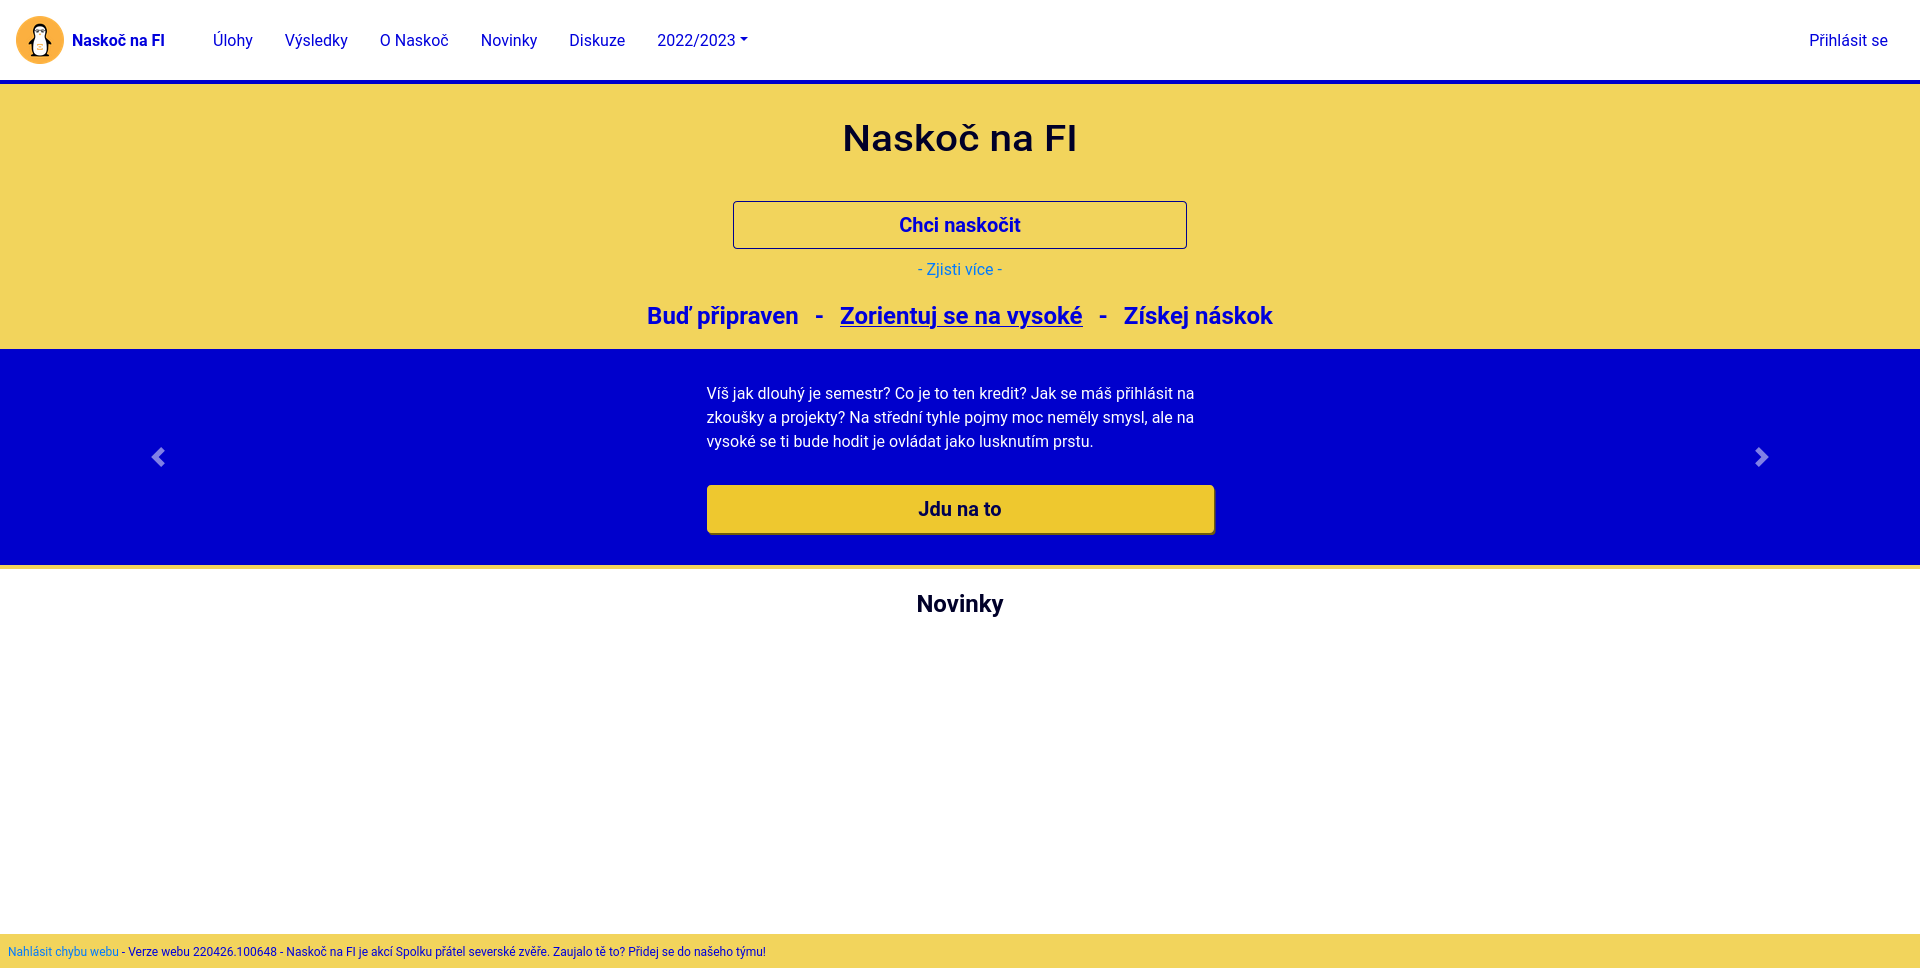
\includegraphics[width=\textwidth]{assets/img/naskoc-na-fi}
\caption{The welcome page for Jump-start the FI}
\label{fig:naskoc-na-fi}
\end{figure}

## Restoring historic OSI tasks

Before OSI was transformed into an online competition, all assignments were sent to the participants through traditional mail. As such, the tasks were written as \LaTeX files, which were then built into a final PDF for printing. This format is incompatible with current tasks which are written as markdown files and then converted to HTML on the backend. Still, these historic tasks have undeniable education value, so making them easily accessible online	was set as one of the secondary goals of this thesis.

Because the backend converts internally the tasks written in markdown to HTML, it is possible to convert the \LaTeX to HTML directly with a tool [`latex2html`](https://www.latex2html.org/), which can be later inserted into the database directly. Whenever `latex2html` encounters a part of a file that it is unable to translate into HTML, instead it renders it as a PNG or SVG image and attaches it to the final HTML file. This operation is also performed on blocks with Tex mathematics and source code, both for which the OSI web has support. The original Tex original mathematic content is obtained from alternative text of respective image from HTML. Additionally, most SVG images created by the tool contain a large transparent margin, which has to be removed. Finally, to contain all assets inside a single HTML file, all images are inserted into the HTML code.

After all tasks are converted into their HTML variants, it is possible to generate a SQL script, which will insert the tasks into the database. The script divides the tasks by their year and wave, while maintaining their relative order by using OSI prerequisites. If the source task was assigned a number of points, a module for submitting solution with correct points will be shown.

Currently, the tasks are accessible only through the public development OSI instance -- for example the task ["Atlas"](https://ksi.ahlava.cz/ulohy/183) from the fifth wave of the 2009 year. Before deploying these historic tasks on the production server a larger discussion with the OSI organizers teams is needed, as follow up tasks, such as creating icons, may be required first. This discussion is planned on the summer or 2022. The source code of this converter is [publicly available](https://github.com/fi-ksi/seminar-till-2014-converter).

## Evaluating the new web application

Since the October 2021 the OSI organizers were encouraged to submit their feedback on the state of the new web frontend. The new frontned was scheduled to be made public with a release of the last wave of the OSI year 2021/2022. Up until that date, the organizers have submitted through designated form 9 bug reports and 10 feature suggestions. With the release of the last fourth wave of the OSI year 2021/2022, the feedback was opened also to the participants, together with a questionnaire for them to fill. The participants were motivated to fill the questionnaire by awarding a trophy to everyone who submits it.

### Questionare

The questionare sent to the OSI participants consisted of three parts. In the first part, the participants were asked to provide their opinion on two new experimental UX features. The second section has consisted of questions about comparsion of the new and current OSI web frontend. The last section was made of free form questions about what do participants think that has improved with a new web and what was better on the current web frontend. As the answers, the participants were asked to choose a number between 1 and 5, where 1 is the best and 5 is the worst. A total of 21 participants have submitted the form.

#### Respondents and responsiveness

Most participants who submitted the questionare have tested the new web on both desktop computer and mobile device (81 \%, \autoref{fig:q-device}). The total of 57.2 \% respondents have answered, that the new web application is faster than the current one, 38.1 \% considers the responsiveness of both frontends to be on a similar level (\autoref{fig:q-speed}).

\begin{figure}
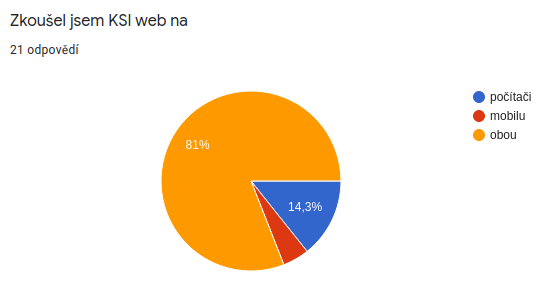
\includegraphics[width=\textwidth]{assets/img/questionare/device}
\caption{Questionare: Used devices devices -- blue for desktop computer only, red for mobile only and orange for both}
\label{fig:q-device}
\end{figure}

\begin{figure}
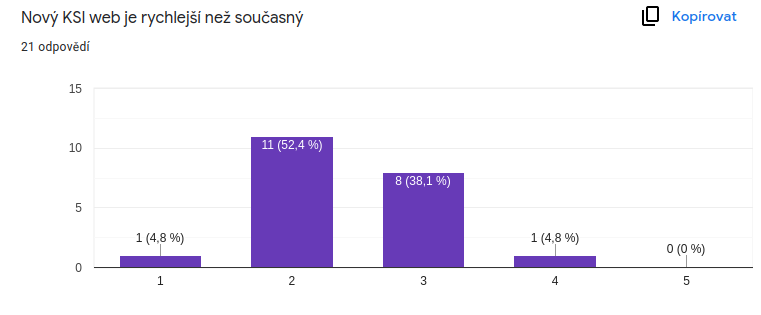
\includegraphics[width=\textwidth]{assets/img/questionare/faster}
\caption{Questionare: I find the new OSI web faster than the current}
\label{fig:q-speed}
\end{figure}


#### User experience and user interface design

Even though most participants agree that the UX and UI on the desktop is better or the same (81 \%, \autoref{fig:q-ux-pc}; 95.2 \%, \autoref{fig:q-ui-pc}), the difference is most notable on the mobile phone. For the mobile version, the total of 90.5 \% for the UX (\autoref{fig:q-ux-mobile}) and  85.7 \% for the UI (\autoref{fig:q-ui-mobile}) thinks that the new web application is better than the current one.

\begin{figure}
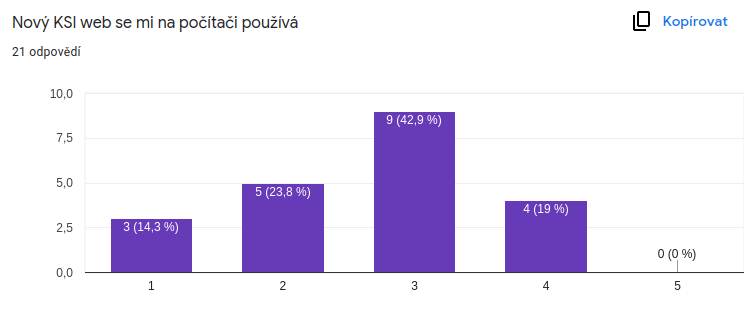
\includegraphics[width=\textwidth]{assets/img/questionare/pc-ux}
\caption{Questionare: My experience with the new OSI web on desktop is better}
\label{fig:q-ux-pc}
\end{figure}

\begin{figure}
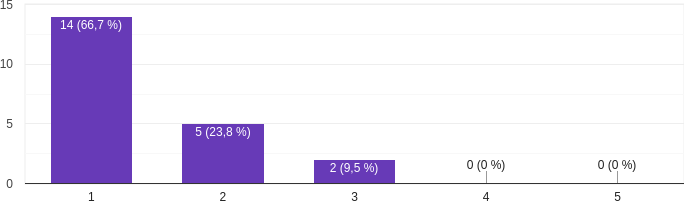
\includegraphics[width=\textwidth]{assets/img/questionare/mobile-ux}
\caption{Questionare: My experience with the new OSI web on mobile is better}
\label{fig:q-ux-mobile}
\end{figure}

\begin{figure}
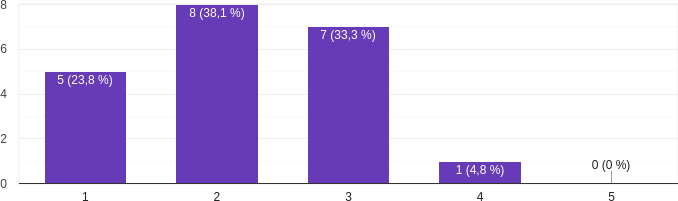
\includegraphics[width=\textwidth]{assets/img/questionare/pc-ui}
\caption{Questionare: The design of the new OSI web interface on desktop is better}
\label{fig:q-ui-pc}
\end{figure}

\begin{figure}
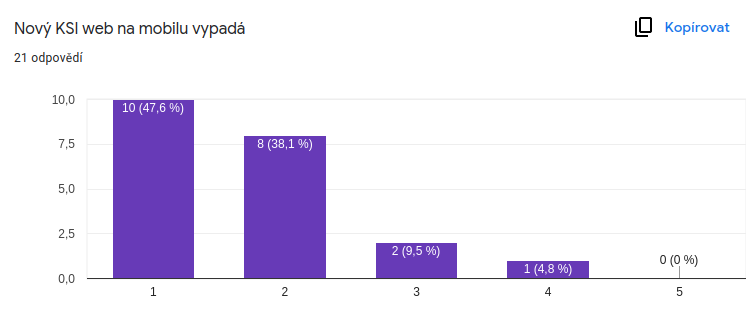
\includegraphics[width=\textwidth]{assets/img/questionare/mobile-ui}
\caption{Questionare: The design of the new OSI web interface on mobile is better}
\label{fig:q-ui-mobile}
\end{figure}



\end{markdown*}

\shorthandon{-}

  \printbibliography[heading=bibintoc] %% Print the bibliography.

  \makeatletter\thesis@blocks@clear\makeatother
  \phantomsection %% Print the index and insert it into the
  \addcontentsline{toc}{chapter}{\indexname} %% table of contents.
  \printindex

\appendix %% Start the appendices.
\chapter{An appendix}
Here you can insert the appendices of your thesis.

\end{document}
